%%%%%%%%%%%%%%%%%%%%%%%%%%%%%%%%%%%%%%%%%%%%%%%%%%%%%%%%%%%%%%%%%%%%%%%%%%%%%%%%%%%%%%%%
%%%%%%%%%%%%%%%%%%%%%%%%%%%%%%%%%%%%%%%%%%%%%%%%%%%%%%%%%%%%%%%%%%%%%%%%%%%%%%%%%%%%%%%%
%%                                                                                    %%
%%               MASTER THESIS - GIOVANNI MANFREDI - 2024 - KTH                       %%
%%                                                                                    %%
%%%%%%%%%%%%%%%%%%%%%%%%%%%%%%%%%%%%%%%%%%%%%%%%%%%%%%%%%%%%%%%%%%%%%%%%%%%%%%%%%%%%%%%%
%%%%%%%%%%%%%%%%%%%%%%%%%%%%%%%%%%%%%%%%%%%%%%%%%%%%%%%%%%%%%%%%%%%%%%%%%%%%%%%%%%%%%%%%
%%
%%%%%%%%%%%%%%%%%%%%%%%%%%%%%%%%%%%%%%%%%%%%%%%%%%%%%%%%%%%%%%%%%%%%%%%%%%%%%%%%%%%%%%%%
%%                                PREAMBLE
%%%%%%%%%%%%%%%%%%%%%%%%%%%%%%%%%%%%%%%%%%%%%%%%%%%%%%%%%%%%%%%%%%%%%%%%%%%%%%%%%%%%%%%%
%%
%% INFORMATION ON THIS PREAMBLE:
%%
%% forked from https://gits-15.sys.kth.se/giampi/kthlatex kthlatex-0.2rc4 on 2020-02-13
%% expanded upon by Gerald Q. Maguire Jr.
%% This template has been adapted by Anders Sjögren to the University
%% Engineering Program in Computer Science at KTH ICT. This adaptation was to
%% translation of English headings into Swedish as the addition of Swedish.
%% Many thanks to others who have provided constructive input regarding the template.

%% Make it possible to conditionally depend on the TeX engine used
\RequirePackage{ifxetex}
\RequirePackage{ifluatex}
\newif\ifxeorlua
\ifxetex\xeorluatrue\fi
\ifluatex\xeorluatrue\fi

\ifxeorlua
%% The following is to ensure that the PDF uses a recent version rather than the typical PDF 1-5
%% This same version of PDF should be set as an option for hyperef

\RequirePackage{expl3}
\ExplSyntaxOn
%pdf_version_gset:n{2.0}
%\pdf_version_gset:n{1.5}

%% Alternatively, if you have a LaTeX newer than June 2022, you can use the following. However, then you have to remove the pdfversion from hyperef. It also breaks hyperxmp. So perhaps it is too early to try using it!
%\DocumentMetadata
%{
%% testphase = phase-I, % tagging without paragraph tagging
% testphase = phase-II % tagging with paragraph tagging and other new stuff.
%pdfversion = 2.0 % pdfversion must be set here.
%}

%% Optionally, you can set the uncompress flag to make it easier to examine the PDF
%\pdf_uncompress: % to check the pdf
\ExplSyntaxOff
\else
\RequirePackage{expl3}
\ExplSyntaxOn
%\pdf_version_gset:n{2.0}
\pdf_version_gset:n{1.5}
\ExplSyntaxOff
\fi


%%%%%%%%%%%%%%%%%%%%%%%%%%%%%%%%%%%%%%%%%%%%%%%%%%%%%%%%%%%%%%%%%%%%%%%%%%%%%%%%%%%%%%%%
%%                              DOCUMENT CLASS
%%%%%%%%%%%%%%%%%%%%%%%%%%%%%%%%%%%%%%%%%%%%%%%%%%%%%%%%%%%%%%%%%%%%%%%%%%%%%%%%%%%%%%%%
%% The template is designed to handle a thesis in English or Swedish
%% set the default language to english or swedish by passing an option to the documentclass - this handles the inside tile page
%% To optimize for digital output (this changes the color palette add the option: digitaloutput
%% To use \ifnomenclature add the option nomenclature
%% To use bibtex or biblatex - include one of these as an option
\documentclass[nomenclature, english, bibtex]{kththesis}
%\documentclass[swedish, biblatex]{kththesis}
% if pdflatex \usepackage[utf8]{inputenc}

%%%%%%%%%%%%%%%%%%%%%%%%%%%%%%%%%%%%%%%%%%%%%%%%%%%%%%%%%%%%%%%%%%%%%%%%%%%%%%%%%%%%%%%%
%%                                 TODO NOTES
%%%%%%%%%%%%%%%%%%%%%%%%%%%%%%%%%%%%%%%%%%%%%%%%%%%%%%%%%%%%%%%%%%%%%%%%%%%%%%%%%%%%%%%%
%% Conventions for todo notes:
%% Informational
%% \generalExpl{Comments/directions/... in English}
\newcommand*{\generalExpl}[1]{\todo[inline]{#1}}                

%% Language-specific information (currently in English or Swedish)
\newcommand*{\engExpl}[1]{\todo[inline, backgroundcolor=kth-lightgreen40]{#1}} %% \engExpl{English descriptions about formatting}
\newcommand*{\sweExpl}[1]{\todo[inline, backgroundcolor=kth-lightblue40]{#1}}  %% % \sweExpl{Text på svenska}

%% warnings
\newcommand*{\warningExpl}[1]{\todo[inline, backgroundcolor=kth-lightred40]{#1}} %% \warningExpl{warnings}

%% Uncomment to hide specific comments, to hide **all** ToDos add `final` to
%% document class
% \renewcommand\warningExpl[1]{}
% \renewcommand\generalExpl[1]{}
% \renewcommand\engExpl[1]{}
%% For example uncommenting the following line hides the Swedish language explanations
% \renewcommand\sweExpl[1]{}

%%%%%%%%%%%%%%%%%%%%%%%%%%%%%%%%%%%%%%%%%%%%%%%%%%%%%%%%%%%%%%%%%%%%%%%%%%%%%%%%%%%%%%%%
%%                               BIBLIOGRAPHY STYLE
%%%%%%%%%%%%%%%%%%%%%%%%%%%%%%%%%%%%%%%%%%%%%%%%%%%%%%%%%%%%%%%%%%%%%%%%%%%%%%%%%%%%%%%%
% \usepackage[style=numeric,sorting=none,backend=biber]{biblatex}
\ifbiblatex
    %\usepackage[language=english,bibstyle=authoryear,citestyle=authoryear, maxbibnames=99]{biblatex}
    %% alternatively you might use another style, such as IEEE and use citestyle=numeric-comp  to put multiple citations in a single pair of square brackets
    \usepackage[style=ieee,citestyle=numeric-comp]{biblatex}
    \addbibresource{references.bib}
    %\DeclareLanguageMapping{norsk}{norwegian}
\else
    %% The line(s) below are for BibTeX
    \bibliographystyle{bibstyle/myIEEEtran}
    %\bibliographystyle{apalike}
\fi

%%%%%%%%%%%%%%%%%%%%%%%%%%%%%%%%%%%%%%%%%%%%%%%%%%%%%%%%%%%%%%%%%%%%%%%%%%%%%%%%%%%%%%%%
%%                             INCLUDES /LIB PACKAGES
%%%%%%%%%%%%%%%%%%%%%%%%%%%%%%%%%%%%%%%%%%%%%%%%%%%%%%%%%%%%%%%%%%%%%%%%%%%%%%%%%%%%%%%%
%% include a variety of packages that are useful
%%%%%%%%%%%%%%%%%%%%%%%%%%%%%% Packages %%%%%%%%%%%%%%%%%%%%%%%%%%%%%%
% The following is for use with the KTH cover when not using XeLaTeX or LuaLaTeX
\ifxeorlua\relax
\else
\usepackage[scaled]{helvet}
\fi

%% The following are needed for generating the DiVA page(s)
\usepackage[force-eol=true]{scontents}              %% Needed to save lang, abstract, and keywords
\usepackage{pgffor}                 %% includes the foreach loop

%% Basic packages

%% Links
\usepackage{xurl}                %% Support for breaking URLs

%% Colorize
%\usepackage{color}
\PassOptionsToPackage{dvipsnames, svgnames, table}{xcolor}
\usepackage{xcolor}

\usepackage[normalem]{ulem}
\usepackage{soul}
\usepackage{xspace}
\usepackage{braket}

% to support units and decimal aligned columns in tables
\usepackage[locale=US]{siunitx}

\usepackage{balance}
\usepackage{stmaryrd}
\usepackage{booktabs}
\usepackage{graphicx}	        %% Support for images
\usepackage{multirow}	        %% Support for multirow columns in tables
\usepackage{tabularx}		    %% For simple table stretching
\usepackage{mathtools}
\usepackage{algorithm} 
\usepackage{algorithmic}  
\usepackage{amsmath}
\usepackage[linesnumbered,ruled,vlined,algo2e]{algorithm2e}
% can't use both algpseudocode and algorithmic packages
%\usepackage[noend]{algpseudocode}
%\usepackage{subfig}  %% cannot use both subcaption and subfig packages
\usepackage{subcaption}
\usepackage{optidef}
\usepackage{float}		        %% Support for more flexible floating box positioning
\usepackage{pifont}

%% some additional useful packages
% to enable rotated figures
\usepackage{rotating}	    	%% For text rotating
\usepackage{array}		        %% For table wrapping
\usepackage{mdwlist}            %% various list-related commands
\usepackage{setspace}           %% For fine-grained control over line spacing


\usepackage{enumitem}           %% to allow changes to the margins of descriptions


%% If you are going to include source code (or code snippets) you can use minted in a listings environment
\usepackage{listings}		    %% For source code listing
                                %% For source code highlighting
%\usepackage[chapter, cache=false]{minted}   %% If you use minted make sure to use the chapter options to do numbering in the chapter
%%\usemintedstyle{borland}

\usepackage{bytefield}          %% For packet drawings


\setlength {\marginparwidth }{2cm} %leave some extra space for todo notes
% The obeyFinal option means that todonotes will be disables when "final" is added as an option for the documentclass
\usepackage[obeyFinal]{todonotes}
\usepackage{notoccite} % do not number captions based on their appearance in the TOC


% Footnotes
\usepackage{perpage}
\usepackage[perpage,symbol]{footmisc} %% use symbols to ``number'' footnotes and reset which symbol is used first on each page
%% Removed option "para" to place each footnote on a separate line. This avoids bad stretching of URLs in footnotes.


%% Various useful packages
%%----------------------------------------------------------------------------
%%   pcap2tex stuff
%%----------------------------------------------------------------------------
\usepackage{tikz}
\usepackage{colortbl}
\usetikzlibrary{arrows,decorations.pathmorphing,backgrounds,fit,positioning, decorations.pathreplacing, calc,shapes, patterns}
\usepackage{pgfmath}	% --math engine
\newcommand\bmmax{2}
\usepackage{bm} % bold math


%% Managing titles
% \usepackage[outermarks]{titlesec}
%%%%%%%%%%%%%%%%%%%%%%%%%%%%%%%%%%%%%%%%%%%%%%%%%%%%%%%%%%%%%%%%%%%%%%
%\captionsetup[subfloat]{listofformat=parens}

% to include PDF pages
%\usepackage{pdfpages}

\usepackage{fvextra}
\usepackage{csquotes}               %% Recommended by biblatex
% to provide a float barrier use:
\usepackage{placeins}

\usepackage{comment}  %% Provides a comment environment
\usepackage{refcount}   %% to be able to get an expandable \getpagerefnumber

% for experiments with new cover
\usepackage{eso-pic}
\usepackage[absolute,overlay]{textpos}

% when the package is used, it draws boxes on the page showing the text, footnote, header, and margin regions of the page
%\usepackage{showframe}  
%\usepackage{printlen} % defines the printlength command to print out values of latex variable

\usepackage{xparse}  % to use for commands with optional arguments

\ifnomenclature
\usepackage[nocfg]{nomencl}  %% include refpage, refeq, to have page number and equation number for each nomenclature
\fi

\usepackage{longtable}  % For multipage tables
\usepackage{lscape}     % For landscape pages
\usepackage{needspace}  % to specify needed space, for example to keep listing heading with the listing
\usepackage{metalogo}   % for \XeLaTeX and \LuaLaTeX logos

% to define a command\B to bold font entries in a table
% based on https://tex.stackexchange.com/questions/469559/bold-entries-in-table-with-s-column-type
\usepackage{etoolbox}
\renewcommand{\bfseries}{\fontseries{b}\selectfont}
\robustify\bfseries
\newrobustcmd{\B}{\bfseries}

% To be able to have conditional text #2 that will be included IFF a label is defined, else #3
\newcommand{\iflabelexists}[3]{\ifcsundef{r@#1}{#3}{#2}}


% to allow more than 16 files to be open at once
% Package morewrites Warning: The morewrites package is unnecessary in LuaTeX.
\ifluatex\empty
\else
\usepackage{morewrites}
\fi

%%% The lines below are for use with the pgfplots examples

\usepackage{svg}
\usepackage{pgfplots}
\usepackage{pgfplotstable}
 \pgfplotsset{compat=1.12}
 

 
%https://tex.stackexchange.com/questions/554732/bar-plot-does-not-use-defined-color-cycle-list
%\pgfplotscreateplotcyclelist{mycolors}{
%    {blue,fill=blue!30!white,mark=none},
%    {green,fill=green!30!white,mark=none},
%    {brown!60!black,fill=brown!30!white,mark=none},
%    {black,fill=gray,mark=none}
%}

    \tikzset{
        hatch distance/.store in=\hatchdistance,
        hatch distance=10pt,
        hatch thickness/.store in=\hatchthickness,
        hatch thickness=2pt
    }

    \makeatletter
    \pgfdeclarepatternformonly[\hatchdistance,\hatchthickness]{flexible hatch}
    {\pgfqpoint{0pt}{0pt}}
    {\pgfqpoint{\hatchdistance}{\hatchdistance}}
    {\pgfpoint{\hatchdistance-1pt}{\hatchdistance-1pt}}%
    {
        \pgfsetcolor{\tikz@pattern@color}
        \pgfsetlinewidth{\hatchthickness}
        \pgfpathmoveto{\pgfqpoint{0pt}{0pt}}
        \pgfpathlineto{\pgfqpoint{\hatchdistance}{\hatchdistance}}
        \pgfusepath{stroke}
    }
\makeatother
%\usetikzlibrary{patterns, patterns.meta}
%\usetikzlibrary{decorations.pathreplacing}
% high contrast colors: https://venngage.com/tools/accessible-color-palette-generator

%#1d138a, #ffffff
%#3829bc, #ffffff
%#c44601, #ffffff
%#008e4a, #000000
%#026526, #ffffff
%https://latex-tutorial.com/color-latex/
\definecolor{color1bg}{HTML}{1954a6}
\colorlet{color1bgFill}{color1bg!30!white}
\colorlet{color1bgDarkFill}{color1bg!90!white}

\definecolor{color2bg}{HTML}{24a0d8}
\colorlet{color2bgFill}{color2bg!30!white}
\colorlet{color2bgDarkFill}{color2bg!90!white}

\definecolor{color3bg}{HTML}{d85497}
\colorlet{color3bgFill}{color3bg!30!white}
\colorlet{color3bgDarkFill}{color3bg!90!white}

\definecolor{color4bg}{HTML}{b0c92b}
\colorlet{color4bgFill}{color4bg!30!white}
\colorlet{color4bgDarkFill}{color4bg!90!white}

\definecolor{color5bg}{HTML}{63666a}
\colorlet{color5bgFill}{color5bg!30!white}
\colorlet{color5bgDarkFill}{color5bg!90!white}

\pgfplotscreateplotcyclelist{rustcolors}{
  {color1bg,mark=none, pattern=
  %{flexible hatch}
  {crosshatch}
  ,pattern color=color1bg},
  {color2bg,mark=none, pattern={vertical lines}, pattern color=color2bg},{color3bg,mark=none, pattern={horizontal lines}, pattern color=color3bg},{color4bg,mark=none, pattern={north east lines}, pattern color=color4bg},{color5bg,fill=color5bg,mark=none},
  {black,fill=gray,mark=none}
}

\pgfplotsset{cycle list name=rustcolors}
\pgfplotsset{/pgfplots/bar cycle list/.style={/pgfplots/cycle list name={rustcolors}}}

\usepackage{makecell}

%\usepackage[table]{xcolor}

\usepackage{pgf-pie}

\usetikzlibrary{tikzmark}

%%% The lines below are for setting text that includes Japanese
\ifluatex
\usepackage{luatexja-fontspec}
\setmainjfont{IPAexMincho} % A high quality Japanese font preinstalled in TeX Live
\fi


%%% Manual additions

\usepackage{caption}
\usepackage{subcaption}
\usepackage{graphicx}
\usepackage{mwe}

%% For Python listings
% Default fixed font does not support bold face
\DeclareFixedFont{\ttb}{T1}{txtt}{bx}{n}{12} % for bold
\DeclareFixedFont{\ttm}{T1}{txtt}{m}{n}{12}  % for normal

% Custom colors
\usepackage{color}

% Have figure and table side-by-side
\usepackage{subfloat}

% Decimal point alignment in tables
\usepackage{siunitx}

% To better display TODO: 
% Set this to suppress "underfull boxes" errors
\hbadness=99999  % or any number >=10000
\usepackage{booktabs}
%%% Local Variables:
%%% mode: latex
%%% TeX-master: t
%%% End:
% KTH colors for LaTeX documents
%
% Started from kthcolors by:
% Riccardo Sven Risuleo
% 2016-09-06 11:05:40
%
% from https://github.com/KTH-AC/kthcolors
%
% Adapted using the colors from "Graphic Profile Manual KTH" version 180604
% (i.e.. 2018-06-04) 
% see https://intra.kth.se/en/administration/kommunikation/grafiskprofil/kth-s-grafiska-profil-1.844676
% 
% G. Q. Maguire Jr.
% 2021-07-05
%

%\NeedsTexFormat{LaTeX2e}[1994/06/01]
%\ProvidesPackage{kthcolors}[2021/07/85 v3 Latex package with official KTH colors]

\RequirePackage{xcolor}
%% Primary colors
%% As of the new manual, there is only 1 primary color; but with three 
\definecolor{kth-blue}{RGB/cmyk}{25,84,166/0.849,0.494,0,0.349}
\colorlet{kth-blue80}{kth-blue!80!}
\colorlet{kth-blue40}{kth-blue!40!}

% these are no longer used as of 2018-06-04
%\definecolor{kth-red}{RGB/cmyk}{157,16,45/0,0.898,0.713,0.384}
%\definecolor{kth-green}{RGB/cmyk}{98,146,46/0.329,0,0.685,0.427}

%% Secondary colors
\definecolor{kth-lightblue}{RGB/cmyk}{36,160,216/0.833,0.259,0,0.153}
\colorlet{kth-lightblue80}{kth-lightblue!80!}
\colorlet{kth-lightblue40}{kth-lightblue!40!}

%\definecolor{kth-lightred}{RGB/cmyk}{228,54,62/0,0.763,0.728,0.106}
\definecolor{kth-lightred}{RGB}{216,84,151}
\colorlet{kth-lightred80}{kth-lightred!80!}
\colorlet{kth-lightred40}{kth-lightred!40!}

\definecolor{kth-lightgreen}{RGB/cmyk}{176,201,43/0.124,0,0.786,0.212} % olive
\colorlet{kth-lightgreen80}{kth-lightgreen!80!}
\colorlet{kth-lightgreen40}{kth-lightgreen!40!}

% Cool Gray 9C
%\definecolor{kth-coolgray}{RGB}{101,101,108}

% Cool Gray 10 suggested by Martin Krzywinski (see http://mkweb.bcgsc.ca/colorblind) 
\definecolor{kth-coolgray}{RGB}{99,102,106}
\colorlet{kth-coolgray80}{kth-coolgray!80!}
\colorlet{kth-coolgray40}{kth-coolgray!40!}

% Tertiary colors (yet more colors)
% All of these are no longer used
%\definecolor{kth-pink}{RGB/cmyk}{216,84,151/10,0.611,0.301,0.153}
%\definecolor{kth-yellow}{RGB/cmyk}{250,185,25/0,0.26,0.9,0.0196}
%\definecolor{kth-darkgray}{RGB/cmyk}{101,101,108/0.0648,0.0648,0,0.576}
%\definecolor{kth-middlegray}{RGB/cmyk}{189,188,188/0,0.00529,0.00529,0.259}
%\definecolor{kth-lightgray}{RGB/cmyk}{227,229,227/0.00873,0,0.00873,0.102}

%\DeclareOption{gray}{\colorlet{gray}{kth-darkgray}}

% These versions are designed to meet accessability requirements for digital media
% Note that the palette is more limited than for the print version of the colors
\ifdigitaloutput
    % primary color
    \definecolor{kth-blue}{HTML}{1954A6} % Deep sea
    \definecolor{kth-blue80}{HTML}{5E87C0}

    % Secondary colors
    \definecolor{kth-lightblue}{HTML}{2191C4} % Stratosphere
    \definecolor{kth-lightred}{HTML}{D02F80} % Fluorescence
    \definecolor{kth-lightred80}{HTML}{D95599}
    \definecolor{kth-lightgreen}{HTML}{62922E} % Front-lawn
    \definecolor{kth-coolgray}{HTML}{65656C} % Office
    \definecolor{kth-coolgray80}{HTML}{848489}
\fi



%\glsdisablehyper
%\makeglossaries
%\makenoidxglossaries
%%%% Local Variables:
%%% mode: latex
%%% TeX-master: t
%%% End:
% The following command is used with glossaries-extra
\setabbreviationstyle[acronym]{long-short}
% The form of the entries in this file is \newacronym{label}{acronym}{phrase}
%                                      or \newacronym[options]{label}{acronym}{phrase}
% see "User Manual for glossaries.sty" for the  details about the options, one example is shown below
% note the specification of the long form plural in the line below
\newacronym[longplural={Debugging Information Entities}]{DIE}{DIE}{Debugging Information Entity}
%
% The following example also uses options
\newacronym[shortplural={OSes}, firstplural={operating systems (OSes)}]{OS}{OS}{operating system}

% note the use of a non-breaking dash in long text for the following acronym
\newacronym{IQL}{IQL}{Independent Q‑Learning}

% example of putting in a trademark on first expansion
\newacronym[first={NVIDIA OpenSHMEM Library (NVSHMEM\texttrademark)}]{NVSHMEM}{NVSHMEM}{NVIDIA OpenSHMEM Library}

\newacronym{KTH}{KTH}{KTH Royal Institute of Technology}

\newacronym{LAN}{LAN}{Local Area Network}
\newacronym{VM}{VM}{virtual machine}
% note the use of a non-breaking dash in the following acronym
\newacronym{WiFi}{Wi‑Fi}{Wireless Fidelity}

\newacronym{WLAN}{WLAN}{Wireless Local Area Network}
\newacronym{UN}{UN}{United Nations}
\newacronym{SDG}{SDG}{Sustainable Development Goal}
                %%load the acronyms file

\makeatletter
\newcommand{\DeclareLatinAbbrev}[2]{%
  \DeclareRobustCommand{#1}{%
  \@ifnextchar\cite{\textit{#2.\,}}{%  if next is a \cite then insert a period and a thin space
    \@ifnextchar{.}{\textit{#2}}{%
      \@ifnextchar{,}{\textit{#2.}}{%
        \@ifnextchar{!}{\textit{#2.}}{%
          \@ifnextchar{?}{\textit{#2.}}{%
            \@ifnextchar{)}{\textit{#2.}}{%
              {\textit{#2.,\ }}}}}}}}}%
}
\makeatother
\DeclareLatinAbbrev{\eg}{e.g}
\DeclareLatinAbbrev{\Eg}{E.g}
\DeclareLatinAbbrev{\ie}{i.e}
\DeclareLatinAbbrev{\Ie}{I.e}
\DeclareLatinAbbrev{\etc}{etc}
\DeclareLatinAbbrev{\etal}{et~al}

\def\first {$(i)$\xspace}
\def\Second{$(ii)$\xspace}
\def\third {$(iii)$\xspace}
\def\fourth{$(iv)$\xspace}
\def\fifth {$(v)$\xspace}
\def\sixth {$(vi)$\xspace}
\def\seventh{$(vii)$\xspace}
\def\eighth{$(viii)$\xspace}

%%% custom definitions
%% Coloring the links!
\newcommand\myshade{75} % Usage: red!\myshade!black

\definecolor{ForestGreen} {RGB}{34,  139,  34}
\definecolor{HeraldRed2}   {rgb}{0.81, 0.12, 0.15}

\newcommand{\refscolor} {blue}
\newcommand{\linkscolor}{HeraldRed2}
\newcommand{\urlscolor} {ForestGreen}

%% Some definitions of used colors
%\definecolor{darkblue}{rgb}{0.0,0.0,0.3} %% define a color called darkblue
%\definecolor{darkred}{rgb}{0.4,0.0,0.0}
%\definecolor{red}{rgb}{0.7,0.0,0.0}
%\definecolor{lightgrey}{rgb}{0.8,0.8,0.8} 
%\definecolor{grey}{rgb}{0.6,0.6,0.6}
%\definecolor{darkgrey}{rgb}{0.4,0.4,0.4}
%\definecolor{aqua}{rgb}{0.0, 1.0, 1.0}

% For runin headings
\newcommand{\smartparagraph}[1]{\vspace{.05in}\noindent\textbf{#1}}

%% Table of Contents (ToC) depth 
\setcounter{secnumdepth}{4} % how many sectioning levels to assign numbers to
\setcounter{tocdepth}{4}    % how many sectioning levels to show in ToC

%% Limit hyphenation
\hyphenpenalty=9000
\tolerance=5000
% Reduce hyphenation as much as possible:
%\hyphenpenalty=15000
%\tolerance=1000

% For notes by the authors to themselves
\newcommand*{\todoinline}[1]{\textcolor{red}{TODO: #1}}

%\DeclareUnicodeCharacter{2003}{\quad}

% Use grouping for numbers that are 4 or more digits long
\sisetup{group-minimum-digits=4}

%%% Manual additions

%% For Python listings
\definecolor{deepblue}{rgb}{0,0,0.5}
\definecolor{deepred}{rgb}{0.6,0,0}
\definecolor{deepgreen}{rgb}{0,0.5,0}

% Python style for highlighting
\newcommand\pythonstyle{\lstset{
language=Python,
basicstyle=\ttm,
morekeywords={self},              % Add keywords here
keywordstyle=\ttb\color{deepblue},
emph={MyClass,__init__},          % Custom highlighting
emphstyle=\ttb\color{deepred},    % Custom highlighting style
stringstyle=\color{deepgreen},
frame=tb,                         % Any extra options here
showstringspaces=false
}}

% Python environment
\lstnewenvironment{python}[1][]
{
\pythonstyle
\lstset{#1}
}
{}

% Python for external files
\newcommand\pythonexternal[2][]{{
\pythonstyle
\lstinputlisting[#1]{#2}}}

% Python for inline
\newcommand\pythoninline[1]{{\pythonstyle\lstinline!#1!}}  %% load some additional definitions to make writing more consistent

%%%%%%%%%%%%%%%%%%%%%%%%%%%%%%%%%%%%%%%%%%%%%%%%%%%%%%%%%%%%%%%%%%%%%%%%%%%%%%%%%%%%%%%%
%%                                DIVA COMMANDS
%%%%%%%%%%%%%%%%%%%%%%%%%%%%%%%%%%%%%%%%%%%%%%%%%%%%%%%%%%%%%%%%%%%%%%%%%%%%%%%%%%%%%%%%
%% The following is needed in conjunction with generating the DiVA data with abstracts and keywords using the scontents package and a modified listings environment
%\usepackage{listings}   %%  already included
\ExplSyntaxOn
\newcommand\typestoredx[2]{\expandafter\__scontents_typestored_internal:nn\expandafter{#1} {#2}}
\ExplSyntaxOff
\makeatletter
\let\verbatimsc\@undefined
\let\endverbatimsc\@undefined
\lst@AddToHook{Init}{\hyphenpenalty=50\relax}
\makeatother


\lstnewenvironment{verbatimsc}
    {
    \lstset{%
        basicstyle=\ttfamily\tiny,
        backgroundcolor=\color{white},
        %basicstyle=\tiny,
        %columns=fullflexible,
        columns=[l]fixed,
        language=[LaTeX]TeX,
        %numbers=left,
        %numberstyle=\tiny\color{gray},
        keywordstyle=\color{red},
        breaklines=true,                 %% sets automatic line breaking
        breakatwhitespace=true,          %% sets if automatic breaks should only happen at whitespace
        %keepspaces=false,
        breakindent=0em,
        %fancyvrb=true,
        frame=none,                     %% turn off any box
        postbreak={}                    %% turn off any hook arrow for continuation lines
    }
}{}

%% Add some more keywords to bring out the structure more
\lstdefinestyle{[LaTeX]TeX}{
morekeywords={begin, todo, textbf, textit, texttt}
}

%% definition of new command for bytefield package
\newcommand{\colorbitbox}[3]{%
	\rlap{\bitbox{#2}{\color{#1}\rule{\width}{\height}}}%
	\bitbox{#2}{#3}}


%%%%%%%%%%%%%%%%%%%%%%%%%%%%%%%%%%%%%%%%%%%%%%%%%%%%%%%%%%%%%%%%%%%%%%%%%%%%%%%%%%%%%%%%
%%                             LEFT ALIGNED TABLE CELL
%%%%%%%%%%%%%%%%%%%%%%%%%%%%%%%%%%%%%%%%%%%%%%%%%%%%%%%%%%%%%%%%%%%%%%%%%%%%%%%%%%%%%%%%
%% define a left aligned table cell that is ragged right
\newcolumntype{L}[1]{>{\raggedright\let\newline\\\arraybackslash\hspace{0pt}}p{#1}}

%%%%%%%%%%%%%%%%%%%%%%%%%%%%%%%%%%%%%%%%%%%%%%%%%%%%%%%%%%%%%%%%%%%%%%%%%%%%%%%%%%%%%%%%
%%                         BACKREF BIBLATEX INCOMPATIBILITY
%%%%%%%%%%%%%%%%%%%%%%%%%%%%%%%%%%%%%%%%%%%%%%%%%%%%%%%%%%%%%%%%%%%%%%%%%%%%%%%%%%%%%%%%
%% Because backref is not compatible with biblatex
\ifbiblatex
    \usepackage[plainpages=false]{hyperref}
\else
    \usepackage[
    backref=page,
    pagebackref=false,
    plainpages=false,
                            %% PDF related options
    unicode=true,           %% Unicode encoded PDF strings
    bookmarks=true,         %% generate bookmarks in PDF files
    bookmarksopen=false,    %% Do not automatically open the bookmarks in the PDF reading program
    pdfpagemode=UseNone,    %% None, UseOutlines, UseThumbs, or FullScreen
    destlabel,              %% better naming of destinations
    pdfencoding=auto,       %% for unicode in 
    ]{hyperref}
    \makeatletter
    \ltx@ifpackageloaded{attachfile2}{
    %% cannot use backref if one is using attachfile
    }
    {\usepackage{backref}
    %%
    %% Customize list of backreferences.
    %% From https://tex.stackexchange.com/a/183735/1340
    \renewcommand*{\backref}[1]{}
    \renewcommand*{\backrefalt}[4]{%
    \ifcase #1%
          \or [Page~#2.]%
          \else [Pages~#2.]%
    \fi%
    }
    }
    \makeatother

\fi
\usepackage[all]{hypcap}	%% prevents an issue related to hyperref and caption linking

%%%%%%%%%%%%%%%%%%%%%%%%%%%%%%%%%%%%%%%%%%%%%%%%%%%%%%%%%%%%%%%%%%%%%%%%%%%%%%%%%%%%%%%%
%%                                 ACRONYMS
%%%%%%%%%%%%%%%%%%%%%%%%%%%%%%%%%%%%%%%%%%%%%%%%%%%%%%%%%%%%%%%%%%%%%%%%%%%%%%%%%%%%%%%%
%% note that nonumberlist - removes the cross references to the pages where the acronym appears
%% note that super will set the descriptions text aligned
%% note that nomain - does not produce a main glossary, thus only acronyms will be in the glossary
%% note that nopostdot - will prevent there being a period at the end of each entry
\usepackage[acronym, style=super, section=section, nonumberlist, nomain,
nopostdot]{glossaries}
\setlength{\glsdescwidth}{0.75\textwidth}
\usepackage[automake]{glossaries-extra}
\ifinswedish
    %\usepackage{glossaries-swedish}
\fi

% packages that have to be included after hyperref
\usepackage{doi}
\usepackage{cleveref}           %% Replace Section with a symbol
\usepackage{hyperxmp}           %% to be able to add the copyright information to the PDF metadata

% To be able to attach files to the final PDF
% Note that the package used is attachfile2 and not attachfile - as the former supports most TeX engines
\usepackage{attachfile2}

%% If you are going to set bidirectional text, i.e., left to right and right to left, add bidi as the last package
%\usepackage{bidi}


%%%%%%%%%%%%%%%%%%%%%%%%%%%%%%%%%%%%%%%%%%%%%%%%%%%%%%%%%%%%%%%%%%%%%%%%%%%%%%%%%%%%%%%%
%%                          MAKE GLOSSARIES COMMAND
%%%%%%%%%%%%%%%%%%%%%%%%%%%%%%%%%%%%%%%%%%%%%%%%%%%%%%%%%%%%%%%%%%%%%%%%%%%%%%%%%%%%%%%%
%\glsdisablehyper
\makeglossaries
%\makenoidxglossaries

%%%%%%%%%%%%%%%%%%%%%%%%%%%%%%%%%%%%%%%%%%%%%%%%%%%%%%%%%%%%%%%%%%%%%%%%%%%%%%%%%%%%%%%%
%%                          PDFLaTeX non-breaking hypen problem
%%%%%%%%%%%%%%%%%%%%%%%%%%%%%%%%%%%%%%%%%%%%%%%%%%%%%%%%%%%%%%%%%%%%%%%%%%%%%%%%%%%%%%%%
%% The following bit of ugliness is because of the problems PDFLaTeX has handling a non-breaking hyphen
%% unless it is converted to UTF-8 encoding.
%% If you do not use such characters in your acronyms, this could be simplified to just include the acronyms file.
\ifxeorlua
%%% Local Variables:
%%% mode: latex
%%% TeX-master: t
%%% End:
% The following command is used with glossaries-extra
\setabbreviationstyle[acronym]{long-short}
% The form of the entries in this file is \newacronym{label}{acronym}{phrase}
%                                      or \newacronym[options]{label}{acronym}{phrase}
% see "User Manual for glossaries.sty" for the  details about the options, one example is shown below
% note the specification of the long form plural in the line below
\newacronym[longplural={Debugging Information Entities}]{DIE}{DIE}{Debugging Information Entity}
%
% The following example also uses options
\newacronym[shortplural={OSes}, firstplural={operating systems (OSes)}]{OS}{OS}{operating system}

% note the use of a non-breaking dash in long text for the following acronym
\newacronym{IQL}{IQL}{Independent Q‑Learning}

% example of putting in a trademark on first expansion
\newacronym[first={NVIDIA OpenSHMEM Library (NVSHMEM\texttrademark)}]{NVSHMEM}{NVSHMEM}{NVIDIA OpenSHMEM Library}

\newacronym{KTH}{KTH}{KTH Royal Institute of Technology}

\newacronym{LAN}{LAN}{Local Area Network}
\newacronym{VM}{VM}{virtual machine}
% note the use of a non-breaking dash in the following acronym
\newacronym{WiFi}{Wi‑Fi}{Wireless Fidelity}

\newacronym{WLAN}{WLAN}{Wireless Local Area Network}
\newacronym{UN}{UN}{United Nations}
\newacronym{SDG}{SDG}{Sustainable Development Goal}
                %load the acronyms file
\else
%%% Local Variables:
%%% mode: latex
%%% TeX-master: t
%%% End:
% The following command is used with glossaries-extra
\setabbreviationstyle[acronym]{long-short}
% The form of the entries in this file is \newacronym{label}{acronym}{phrase}
%                                      or \newacronym[options]{label}{acronym}{phrase}
% see "User Manual for glossaries.sty" for the  details

\newacronym{KTH}{KTH}{KTH Royal Institute of Technology}
\newacronym{AB}{AB}{\textit{Aktiebolag}, tr. Limited company}
\newacronym{ACID}{ACID}{Atomicity, Consistency, Isolation and Durability}
\newacronym{AI}{AI}{Artificial Intelligence}
\newacronym{ML}{ML}{Machine Learning}
\newacronym{BI}{BI}{Business Intelligence}
\newacronym[shortplural={RDDs}, firstplural={Resilient Distributed Datasets (RDDs)}]{RDD}{RDD}{Resilient Distributed Dataset}
\newacronym{OLAP}{OLAP}{On-Line Analytical Processing}
\newacronym{ELT}{ELT}{Extract Load Transform}
\newacronym{ETL}{ETL}{Extract Transform Load}
\newacronym{HDFS}{HDFS}{Hadoop Distributed File System}
\newacronym{JVM}{JVM}{Java Virtual Machine}
\newacronym[shortplural={INs}, firstplural={Industrial Needs (INs)}]{IN}{IN}{Industrial Need}
\newacronym[shortplural={PAs}, firstplural={Project Assumptions (PAs)}]{PA}{PA}{Project Assumption}
\newacronym[shortplural={APIs}, firstplural={Application Programming Interfaces (APIs)}]{API}{API}{Application Programming Interface}
\newacronym{OLTP}{OLTP}{On-Line Transaction Processing}
\newacronym[shortplural={DBMs}, firstplural={Data Base Management Systems}]{DBMS}{DBMS}{Data Base Management System}
\newacronym[shortplural={Gs}, firstplural={Goals}]{G}{G}{Goal}
\newacronym[shortplural={RQs}, firstplural={Research Questions}]{RQ}{RQ}{Research Question}
\newacronym[shortplural={Ds}, firstplural={Deliverables}]{D}{D}{Deliverable}
\newacronym{CRUD}{CRUD}{Create Read Update Delete}
\newacronym[shortplural={SDGs}, firstplural={Sustainable Development Goals}]{SDG}{SDG}{Sustainable Development Goal}
\newacronym{AWS}{AWS}{Amazon Web Services}
\newacronym{GCS}{GCS}{Google Cloud Storage}
\newacronym[shortplural={HDDs}, firstplural={Hard Disks Drives}]{HDD}{HDD}{Hard Disk Drive}
\newacronym[shortplural={SSDs}, firstplural={Solid State Drives}]{SSD}{SSD}{Solid State Drive}
\newacronym[shortplural={PCs}, firstplural={Personal Computers}]{PC}{PC}{Personal Computer}
\newacronym[shortplural={OSes}, firstplural={Operating Systems (OSes)}]{OS}{OS}{Operating System}
\newacronym[shortplural={DFSes}, firstplural={Distributed File Systems (DFSes)}]{DFS}{DFS}{Distributed File System}
\newacronym{BPMN}{BPMN}{Business Process Model and Notation}
\newacronym{TLS}{TLS}{Transport Layer Security}
\newacronym{SSH}{SSH}{Secure Shell protocol}
\newacronym{VM}{VM}{Virtual Machine}
\newacronym{CoC}{CoC}{Conquer of Completion}
\newacronym{SF}{SF}{Scale Factor}
\newacronym{CPU}{CPU}{Central Processing Unit}
\newacronym{GPU}{GPU}{Graphical Processing Unit}
\newacronym{HopsFS}{HopsFS}{Hopsworks' \glsentryshort{HDFS} distribution}
\newacronym{LocalFS}{LocalFS}{Local File System}
\newacronym{TPC}{TPC}{Transaction Processing Performance Council}
\newacronym{RAM}{RAM}{Random Access Memory}
\newacronym{RPC}{RPC}{Remote Procedural Call}
\newacronym{CIDR}{CIDR}{Conference on Innovative Data Systems Research}
\newacronym{MLOps}{MLOps}{Machine Learning Operations}
\newacronym{LOC}{LOC}{Lines Of Code}

\fi

%%%%%%%%%%%%%%%%%%%%%%%%%%%%%%%%%%%%%%%%%%%%%%%%%%%%%%%%%%%%%%%%%%%%%%%%%%%%%%%%%%%%%%%%
%%                                    FRONT PAGE
%%%%%%%%%%%%%%%%%%%%%%%%%%%%%%%%%%%%%%%%%%%%%%%%%%%%%%%%%%%%%%%%%%%%%%%%%%%%%%%%%%%%%%%%
%% insert the configuration information with author(s), examiner, supervisor(s), ...
%%%%%%%%%%%%%%%%%%%%%%%%%%%%%%%%%%%%%%%%%%%%%%%%%%%%%%%%%%%%%%%%%%%%%%%%%%%%%%%%%%%%%%%%
%%                        INFORMATION INSIDE TITLE PAGE
%%%%%%%%%%%%%%%%%%%%%%%%%%%%%%%%%%%%%%%%%%%%%%%%%%%%%%%%%%%%%%%%%%%%%%%%%%%%%%%%%%%%%%%%
%%
%% AUTHORS INFO
%%
\authorsLastname{Manfredi}
\authorsFirstname{Fake A.}
\email{a@kth.se}
\kthid{u100001}
%% As per email from KTH Biblioteket on 2021-06-28 students cannot have an OrCiD reported for their degree project
\authorsSchool{\schoolAcronym{EECS}}
%% If the student is not in Stockholm, Sweden, add that information here
%% This information will be used when generating the acknowledgements signature.
%\authorCity{A City}
%\authorCountry{A Country}
%% pass into \authorCityCountryDate{} the month and year for the acknowledgment
%% Specify the month and year for the first author:
\authorCityCountryDate{\MONTH\enspace\the\year}

%%
%% SUPERVISOR INFO
%%
\supervisorAsLastname{Supervisor}
\supervisorAsFirstname{A. Busy}
\supervisorAsEmail{sa@kth.se}
%% If the supervisor is from within KTH add their KTHID, School and Department info
\supervisorAsKTHID{u100003}
\supervisorAsSchool{\schoolAcronym{EECS}}
\supervisorAsDepartment{Computer Science}
%% other for a supervisor outside of KTH add their organization info
%\supervisorAsOrganization{Timbuktu University, Department of Pseudoscience}

%%If there is a second supervisor add them here:
\supervisorBsLastname{Supervisor}
\supervisorBsFirstname{Another Busy}
\supervisorBsEmail{sb@kth.se}
%% If the supervisor is from within KTH add their KTHID, School and Department info
\supervisorBsKTHID{u100003}
\supervisorBsSchool{\schoolAcronym{ABE}}
\supervisorBsDepartment{Architecture}
%% other for a supervisor outside of KTH add their organization info
%\supervisorBsOrganization{Timbuktu University, Department of Pseudoscience}

%%If there is a third supervisor add them here:
\supervisorCsLastname{Supervisor}
\supervisorCsFirstname{Third Busy}
\supervisorCsEmail{sc@tu.va}
%% If the supervisor is from within KTH add their KTHID, School and Department info
%\supervisorCsKTHID{u100004}
%\supervisorCsSchool{\schoolAcronym{ABE}}
%\supervisorCsDepartment{Public Buildings}
% other for a supervisor outside of KTH add their organization info
\supervisorCsOrganization{Timbuktu University, Department of Pseudoscience}

%%
%% EXAMINER INFO
%%
\examinersLastname{Maguire Jr.}
\examinersFirstname{Gerald Q.}
\examinersEmail{maguire@kth.se}
%% If the examiner is from within KTH add their KTHID, School and Department info
\examinersKTHID{u1d13i2c}
\examinersSchool{\schoolAcronym{EECS}}
\examinersDepartment{Computer Science}
%% other for a examiner outside of KTH add their organization info
%\examinersOrganization{Timbuktu University, Department of Pseudoscience}


\hostcompany{Företaget AB} % Remove this line if the project was not done at a host company
%\hostorganization{CERN}   % if there was a host organization

\date{\today}

%%
%% COURSE INFO
%%
\courseCycle{1}
\courseCode{IA150X}
\courseCredits{15.0}

\programcode{TCOMK}
\degreeName{Bachelors degree}
%% Note that the subject area for a Bachelor's thesis (Kandidatexamen) should be either Technology or Architecture
%% If the thesis is in Swedish, these would be: teknik | arkitektur -- Note the use of lower case
\subjectArea{Technology}
%% if there is a second degree
%\secondProgramcode{CINTE}
%\secondDegreeName{test second degree}
%\secondSubjectArea{test second subject area}

%% Note that in the case of both Both Degree of Master of Science in Engineering and Master's degree
%% there are two cases: "Both" is used when the field of technology (\subjectArea{}) and the main subject (\secondSubjectArea{} are different and the case "Same" when they are the same.
%% Both case
%\courseCycle{2}
%\courseCode{xxxxxx}
%\courseCredits{30.0}
%\degreeName{Both Degree of Master of Science in Engineering and Master's degree}
%\subjectArea{Biotechnology}
%\secondSubjectArea{Medical Engineering}

%\courseCycle{2}
%\courseCode{xxxxxx}
%\courseCredits{30.0}
%\degreeName{Både civilingenjörsexamen och masterexamen}
%\subjectArea{bioteknik}
%\secondSubjectArea{medicinsk teknik}

%% Same case
%\courseCycle{2}
%\courseCode{xxxxxx}
%\courseCredits{30.0}
%\degreeName{Both Degree of Master of Science in Engineering and Master's degree}
%\subjectArea{Biotechnology}
%\secondSubjectArea{Biotechnology}

%\courseCycle{2}
%\courseCode{xxxxxx}
%\courseCredits{30.0}
%\degreeName{Både civilingenjörsexamen och masterexamen}
%\subjectArea{bioteknik}
%\secondSubjectArea{bioteknik}

%% For a CDATE student the following are likely values:
%\programcode{CDATE}
%\courseCycle{2}
%\courseCode{DA231X}
%\courseCredits{30.0}
%\degreeName{Degree of Master of Science in Engineering}
%\subjectArea{Computer Science and Engineering}

%% For a TCSCM student the following are likely values:
%\programcode{TCSCM}
%\courseCycle{2}
%\courseCode{DA231X}
%\courseCredits{30.0}
%\degreeName{Master's Programme, Computer Science, 120 credits}
%\subjectArea{Computer Science}

%% For a CMETE student the following are likely values:
%\programcode{CMETE}
%\courseCycle{2}
%\courseCode{DA231X}
%\courseCredits{30.0}
%\degreeName{Degree of Master of Science in Engineering}
%\subjectArea{Media Technology}

%% For a CINTE student the following are likely values:
%\programcode{CINTE}
%\courseCycle{2}
%\courseCode{DA231X}
%\courseCredits{30.0}
%\degreeName{Degree of Master of Science in Engineering}
%\subjectArea{Information and Communication Technology}


%%%%% for DiVA's National Subject Category information
%%% Enter one or more 3 or 5 digit codes
%%% See https://www.scb.se/contentassets/3a12f556522d4bdc887c4838a37c7ec7/standard-for-svensk-indelning--av-forskningsamnen-2011-uppdaterad-aug-2016.pdf
%%% See https://www.scb.se/contentassets/10054f2ef27c437884e8cde0d38b9cc4/oversattningsnyckel-forskningsamnen.pdf
%%%%
%%%% Some examples of these codes are shown below:
% 102 Data- och informationsvetenskap (Datateknik)    Computer and Information Sciences
% 10201 Datavetenskap (datalogi) Computer Sciences 
% 10202 Systemvetenskap, informationssystem och informatik (samhällsvetenskaplig inriktning under 50804)
% Information Systems (Social aspects to be 50804)
% 10203 Bioinformatik (beräkningsbiologi) (tillämpningar under 10610)
% Bioinformatics (Computational Biology) (applications to be 10610)
% 10204 Människa-datorinteraktion (interaktionsdesign) (Samhällsvetenskapliga aspekter under 50803) Human Computer Interaction (Social aspects to be 50803)
% 10205 Programvaruteknik Software Engineering
% 10206 Datorteknik Computer Engineering
% 10207 Datorseende och robotik (autonoma system) Computer Vision and Robotics (Autonomous Systems)
% 10208 Språkteknologi (språkvetenskaplig databehandling) Language Technology (Computational Linguistics)
% 10209 Medieteknik Media and Communication Technology
% 10299 Annan data- och informationsvetenskap Other Computer and Information Science
%%%
% 202 Elektroteknik och elektronik Electrical Engineering, Electronic Engineering, Information Engineering
% 20201 Robotteknik och automation Robotics
% 20202 Reglerteknik Control Engineering
% 20203 Kommunikationssystem Communication Systems
% 20204 Telekommunikation Telecommunications
% 20205 Signalbehandling Signal Processing
% 20206 Datorsystem Computer Systems
% 20207 Inbäddad systemteknik Embedded Systems
% 20299 Annan elektroteknik och elektronik Other Electrical Engineering, Electronic Engineering, Information Engineering
%% Example for a thesis in Computer Science and Computer Systems
\nationalsubjectcategories{10201, 10206}

%%%%%%%%%%%%%%%%%%%%%%%%%%%%%%%%%%%%%%%%%%%%%%%%%%%%%%%%%%%%%%%%%%%%%%%%%%%%%%%%%%%%%%%%
%%                        TITLE OF TITLE PAGE
%%%%%%%%%%%%%%%%%%%%%%%%%%%%%%%%%%%%%%%%%%%%%%%%%%%%%%%%%%%%%%%%%%%%%%%%%%%%%%%%%%%%%%%%
\title{This is the title in the language of the thesis}
\subtitle{A subtitle in the language of the thesis}

%% give the alternative title - i.e., if the thesis is in English, then give a Swedish title
\alttitle{Detta är den svenska översättningen av titeln}
\altsubtitle{Detta är den svenska översättningen av undertiteln}
%% alternative, if the thesis is in Swedish, then give an English title
%\alttitle{This is the English translation of the title}
%\altsubtitle{This is the English translation of the subtitle}

%% Enter the English and Swedish keywords here for use in the PDF meta data _and_ for later use
%% following the respective abstract.
%% Try to put the words in the same order in both languages to facilitate matching. For example:
\EnglishKeywords{Canvas Learning Management System, Docker containers, Performance tuning}
\SwedishKeywords{Canvas Lärplattform, Dockerbehållare, Prestandajustering}

%%%%% For the oral presentation
%% Add this information once your examiner has scheduled your oral presentation
\presentationDateAndTimeISO{2022-03-15 13:00}
\presentationLanguage{eng}
\presentationRoom{via Zoom https://kth-se.zoom.us/j/ddddddddddd}
\presentationAddress{Isafjordsgatan 22 (Kistagången 16)}
\presentationCity{Stockholm}

%% When there are multiple opponents, separate their names with '\&'
%% Opponent's information
\opponentsNames{A. B. Normal \& A. X. E. Normalè}

%% Once a thesis is approved by the examiner, add the TRITA number
%% The TRITA number for a thesis consists of two parts a series (unique to each school)
%% and the number in the series which is formatted as the year followed by a colon and
%% then a unique series number for the thesis - starting with 1 each year.
\trita{TRITA-EECS-EX}{2023:0000}

%% Put the title, author, and keyword information into the PDF meta information
% This file contains the LaTeX to add information to the PDF file (specifically, author(s), title(s), and keywords
% It uses the hyperref package and should be included before the \begin{document}
%
% I want to acknowledge the inspiration of Karl Voit's template for TU Graz that inspired me to add the PDF document information
% For more information about his template see https://github.com/novoid/LaTeX-KOMA-template
% Note that this template does not use anything from his template other than the names of the information for the PDF meta fields, i.e., mytitle, myauthor, and mykeywords together with the idea of defining the corresponding newcommand to set the relevant hyperref parameters.

\makeatletter
\ifx\@subtitle\@empty
    \newcommand{\mytitle}{\@title}
\else
    \ifinswedish
        \newcommand{\mytitle}{\@title\xspace–\xspace\@subtitle}
    \else
        \newcommand{\mytitle}{\@title: \@subtitle}
    \fi
\fi
\makeatother

% Put the alternative title (and subtitle) into the PDF Subject meta
\makeatletter
\ifx\@altsubtitle\@empty\relax
    \newcommand{\myalttitle}{\@alttitle}
\else
    \ifinswedish
        \newcommand{\myalttitle}{\@alttitle: \@altsubtitle}
    \else
    \newcommand{\myalttitle}{\@alttitle\xspace–\xspace\@altsubtitle}
    \fi
    
\fi
\makeatother
\hypersetup{
     pdfsubject={\myalttitle}        % Subject field
}

\ifinswedish
\XMPLangAlt{en}{pdfsubject={\myalttitle}}
\else
\XMPLangAlt{sv}{pdfsubject={\myalttitle}}
\fi


\ifinswedish
\hypersetup{%
    pdflang={sv},
    pdfmetalang={sv},
    pdftitle={\mytitle}        % Title field
}
\XMPLangAlt{en}{pdftitle={\myalttitle}}
\else
\hypersetup{%
    pdflang={en},
    pdfmetalang={en},
    pdftitle={\mytitle}        % Title field
}
\XMPLangAlt{sv}{pdftitle={\myalttitle}}
\fi

\makeatletter
\ltx@ifpackageloaded{hyperxmp}{
\ifx\@secondAuthorsLastname\@empty
% Note that \hyxmp@comma is used explicitly rather than \xmpcomma
% As the later will simply turn into a comma in this context.
\StrSubstitute{\@authorsLastname}{,}{\hyxmp@comma}[\@authorsLastnameXMP]
    \newcommand{\myauthor}{\xmpquote{\@authorsFirstname\space\@authorsLastnameXMP}} 
\else
% Note that \hyxmp@comma is used explicitly rather than \xmpcomma
% As the later will simply turn into a comma in this context.
\StrSubstitute{\@authorsLastname}{,}{\hyxmp@comma}[\@authorsLastnameXMP]
\StrSubstitute{\@secondAuthorsLastname}{,}{\hyxmp@comma}[\@secondAuthorsLastnameXMP]
    \newcommand{\myauthor}{\xmpquote{\@authorsFirstname\space\@authorsLastnameXMP},
\xmpquote{\@secondAuthorsFirstname\space\@secondAuthorsLastnameXMP}}
\fi
}{
\ifx\@secondAuthorsLastname\@empty
    \newcommand{\myauthor}{\@authorsFirstname\space\@authorsLastname} 
\else
    \newcommand{\myauthor}{\@authorsFirstname\space\@authorsLastname,
\space\@secondAuthorsFirstname\space\@secondAuthorsLastname}
\fi
}% end of ifpackage conditional
\makeatother

\hypersetup{
     pdfauthor={\myauthor}      % Author field
}


\makeatletter
\ifx\@EnglishKeywords\@empty
    \ifx\@SwedishKeywords\@empty
        \newcommand{\mykeywords}{}
    \else
    \newcommand{\mykeywords}{\@SwedishKeywords}
    \fi
\else
    \ifx\@SwedishKeywords\@empty
        \newcommand{\mykeywords}{\@EnglishKeywords}
    \else
        \ifinswedish
            \newcommand{\mykeywords}{\@SwedishKeywords, \@EnglishKeywords}
        \else
            \newcommand{\mykeywords}{\@EnglishKeywords, \@SwedishKeywords}
        \fi
    \fi
\fi
\makeatother

\hypersetup{
     pdfkeywords={\mykeywords}        % Keywords field
}        
% I have _not_ set the following fields:
%    pdfcreator             % Creator field
%    pdfproducer            % Producer field

%% Note that the copyright information is added to the PDF file inside bookinfo{}
%% as until then, the copyright information is unknown.

% Put the alternative title (and subtitle) into the PDF Subject meta
\makeatletter
\ifx\@secondkthid\@empty\relax
    \newcommand{\mykthids}{author: \@kthid}
\else
    \newcommand{\mykthids}{author: \@kthid,\xspace
    secondauthor: \@secondkthid}
\fi
\makeatother

\hypersetup{
     pdfcontactemail={\mykthids}        % Subject field
}

% Add the TRITA number to the metadata
% Get and store information about the series and the number within this series, i.e, TRITA numbers
%"Series": \{
%	"Title of series": "TRITA-ICT-EX"
%	"No. in series": "2019:00"
\makeatletter
\ifinswedish
\hypersetup{
        pdfvolumenum={\@thesisSeries},        % put the series in the volume field
        pdfissuenum={\@thesisSeriesNumber},
        pdfpublisher={Kungliga Tekniska högskolan (KTH)},
        pdfpubtype={report}
}
\else
\hypersetup{
        pdfvolumenum={\@thesisSeries},        % put the series in the volume field
        pdfissuenum={\@thesisSeriesNumber},
        pdfpublisher={KTH Royal Institute of Technology},
        pdfpubtype={report}
}
\fi
\makeatother


% summary

%%%%%%%%%%%%%%%%%%%%%%%%%%%%%%%%%%%%%%%%%%%%%%%%%%%%%%%%%%%%%%%%%%%%%%%%%%%%%%%%%%%%%%%%
%%                                    CUSTOM COLOURS
%%%%%%%%%%%%%%%%%%%%%%%%%%%%%%%%%%%%%%%%%%%%%%%%%%%%%%%%%%%%%%%%%%%%%%%%%%%%%%%%%%%%%%%%
%% the custom colors and the commands are defined in defines.tex    
\hypersetup{
	colorlinks  = true,
	breaklinks  = true,
	linkcolor   = \linkscolor,
	urlcolor    = \urlscolor,
	citecolor   = \refscolor,
	anchorcolor = black
}

%%%%%%%%%%%%%%%%%%%%%%%%%%%%%%%%%%%%%%%%%%%%%%%%%%%%%%%%%%%%%%%%%%%%%%%%%%%%%%%%%%%%%%%%
%%                             NOMENCLATURE (SYMBOL USED)
%%%%%%%%%%%%%%%%%%%%%%%%%%%%%%%%%%%%%%%%%%%%%%%%%%%%%%%%%%%%%%%%%%%%%%%%%%%%%%%%%%%%%%%%
\ifnomenclature
%% The following lines make the page numbers and equations hyperlinks in the Nomenclature list
\renewcommand*{\pagedeclaration}[1]{\unskip, \dotfill\hyperlink{page.#1}{page\nobreakspace#1}}
%% The following does not work correctly, as the name of the cross-reference is incorrect
%\renewcommand*{\eqdeclaration}[1]{, see equation\nobreakspace(\hyperlink{equation.#1}{#1})}

%% You can also change the page heading for the nomenclature
\renewcommand{\nomname}{List of Symbols Used}

%% You can even add customization text before the list
\renewcommand{\nompreamble}{The following symbols will be later used within the body of the thesis.}
\makenomenclature
\fi

%%%%%%%%%%%%%%%%%%%%%%%%%%%%%%%%%%%%%%%%%%%%%%%%%%%%%%%%%%%%%%%%%%%%%%%%%%%%%%%%%%%%%%%%
%%                               JSON, XML LISTINGS
%%%%%%%%%%%%%%%%%%%%%%%%%%%%%%%%%%%%%%%%%%%%%%%%%%%%%%%%%%%%%%%%%%%%%%%%%%%%%%%%%%%%%%%%
%% format for JSON listings
\colorlet{punct}{red!60!black}
\definecolor{delim}{RGB}{20,105,176}
\definecolor{numb}{RGB}{106, 109, 32}
\definecolor{string}{RGB}{0, 0, 0}

\lstdefinelanguage{json}{
    numbers=none,
    numberstyle=\small,
    frame=none,
    rulecolor=\color{black},
    showspaces=false,
    showtabs=false,
    breaklines=true,
    postbreak=\raisebox{0ex}[0ex][0ex]{\ensuremath{\color{gray}\hookrightarrow\space}},
    breakatwhitespace=true,
    basicstyle=\ttfamily\small,
    extendedchars=false,
    upquote=true,
    morestring=[b]",
    stringstyle=\color{string},
    literate=
     *{0}{{{\color{numb}0}}}{1}
      {1}{{{\color{numb}1}}}{1}
      {2}{{{\color{numb}2}}}{1}
      {3}{{{\color{numb}3}}}{1}
      {4}{{{\color{numb}4}}}{1}
      {5}{{{\color{numb}5}}}{1}
      {6}{{{\color{numb}6}}}{1}
      {7}{{{\color{numb}7}}}{1}
      {8}{{{\color{numb}8}}}{1}
      {9}{{{\color{numb}9}}}{1}
      {:}{{{\color{punct}{:}}}}{1}
      {,}{{{\color{punct}{,}}}}{1}
      {\{}{{{\color{delim}{\{}}}}{1}
      {\}}{{{\color{delim}{\}}}}}{1}
      {[}{{{\color{delim}{[}}}}{1}
      {]}{{{\color{delim}{]}}}}{1}
      {’}{{\char13}}1,
}

\lstdefinelanguage{XML}
{
  basicstyle=\ttfamily\color{blue}\bfseries\small,
  morestring=[b]",
  morestring=[s]{>}{<},
  morecomment=[s]{<?}{?>},
  stringstyle=\color{black},
  identifierstyle=\color{blue},
  keywordstyle=\color{cyan},
  breaklines=true,
  postbreak=\raisebox{0ex}[0ex][0ex]{\ensuremath{\color{gray}\hookrightarrow\space}},
  breakatwhitespace=true,
  morekeywords={xmlns,version,type}% list your attributes here
}

%% In case you use both listings and lstlistings - this makes them both use the same counter
\makeatletter
\AtBeginDocument{\let\c@listing\c@lstlisting}
\makeatother
\usepackage{subfiles}

%%%%%%%%%%%%%%%%%%%%%%%%%%%%%%%%%%%%%%%%%%%%%%%%%%%%%%%%%%%%%%%%%%%%%%%%%%%%%%%%%%%%%%%%
%%                            CREATIVE COMMONS LICENCE
%%%%%%%%%%%%%%%%%%%%%%%%%%%%%%%%%%%%%%%%%%%%%%%%%%%%%%%%%%%%%%%%%%%%%%%%%%%%%%%%%%%%%%%%
%% To have Creative Commons (CC) license and logos use the doclicense package
%% Note that the lowercase version of the license has to be used in the modifier
%% i.e., one of by, by-nc, by-nd, by-nc-nd, by-sa, by-nc-sa, zero.
%% For background see:
%% https://www.kb.se/samverkan-och-utveckling/oppen-tillgang-och-bibsamkonsortiet/open-access-and-bibsam-consortium/open-access/creative-commons-faq-for-researchers.html
%% https://kib.ki.se/en/publish-analyse/publish-your-article-open-access/open-licence-your-publication-cc
\begin{comment}
\usepackage[
    type={CC},
    %modifier={by-nc-nd},
    %version={4.0},
    modifier={by-nc},
    imagemodifier={-eu-88x31},  % to get Euro symbol rather than Dollar sign
    hyphenation={RaggedRight},
    version={4.0},
    %modifier={zero},
    %version={1.0},
]{doclicense}
\end{comment}

%%%%%%%%%%%%%%%%%%%%%%%%%%%%%%%%%%%%%%%%%%%%%%%%%%%%%%%%%%%%%%%%%%%%%%%%%%%%%%%%%%%%%%%%
%%                                DOCUMENT
%%%%%%%%%%%%%%%%%%%%%%%%%%%%%%%%%%%%%%%%%%%%%%%%%%%%%%%%%%%%%%%%%%%%%%%%%%%%%%%%%%%%%%%%
\begin{document}
%\selectlanguage{swedish}
\selectlanguage{english}

%% Set the numbering for the title page to a numbering series not in the preface or body
\pagenumbering{alph}
\kthcover
\clearpage\thispagestyle{empty}\mbox{} % empty back of front cover
\titlepage

%% If you do not want to have a bookinfo page, comment out the line saying \bookinfopage and add a \cleardoublepage
%% If you want a bookinfo page: you will get a copyright notice, unless you have used the doclicense package in which case you will get a Creative Commons license. To include the doclicense package, uncomment the configuration of this package above and configure it with your choice of license.
\bookinfopage

%% Frontmatter includes the abstracts and table-of-contents
\frontmatter
\setcounter{page}{1}

%%%%%%%%%%%%%%%%%%%%%%%%%%%%%%%%%%%%%%%%%%%%%%%%%%%%%%%%%%%%%%%%%%%%%%%%%%%%%%%%%%%%%%%%
%%                                ABSTRACTS
%%%%%%%%%%%%%%%%%%%%%%%%%%%%%%%%%%%%%%%%%%%%%%%%%%%%%%%%%%%%%%%%%%%%%%%%%%%%%%%%%%%%%%%%
\begin{abstract}
    % The first abstract should be in the language of the thesis.
  \markboth{\abstractname}{}
\begin{scontents}[store-env=lang]
eng
\end{scontents}
%%% The contents of the abstract (between the begin and end of scontents) will be saved in LaTeX format
%%% and output on the page(s) at the end of the thesis with information for DiVA facilitating the correct
%%% entry of the meta data for your thesis.
%%% These page(s) will be removed before the thesis is inserted into DiVA.



\begin{scontents}[store-env=abstracts,print-env=true]
The growing need for efficient data management in Machine Learning (ML) workflows has led to the widespread adoption of feature stores, centralized data platforms that supports feature engineering, model training and prediction inference. The Hopsworks' feature store has demonstrated outperformance compared to its alternatives, leveraging Apache Hudi and Spark for offline data storage, but suffers from high write and read latency, even for small quantities of data (1GB or less). This thesis explores the potential of Apache Iceberg as an alternative table format, integrating it with HopsFS (Hopsworks HDFS distribution) and PyIceberg Python library to reduce latencies.

The research begin with an evaluation of potential system integration alternatives, documenting the advantages and limitations of each approach. Then, a PyIceberg-based architecture is implemented and evaluated, benchmarking it against the existing Spark-based solution and an alternative Delta Lake implementation (delta-rs). Extensive experiments were conducted across varying table sizes and CPU configurations to assess write and read performance. Results show that PyIceberg significantly reduces write latency -- from 40 to 140 times lower than the legacy system -- and read latency -- from 55\% to 60 times lower than the legacy system. Compared to delta-rs, PyIceberg demonstrates reduced write latency for large tables -- up to 7 times lower -- and equal read latency, but exhibits lower scaling benefits with additional CPU cores -- 20\% less than delta-rs.

These findings confirm that alternatives to Spark-based pipelines in small-scale scenarios are possible and are worth of further investigations, and the system implemented will be included in the Hopsworks feature store. Furthermore, this thesis work and results finally provides a baseline for future work about additional open table formats, alternative languages to mitigate Python's performance overhead, and strategies to improve resource utilization in data management platforms.

% Describe the following:
% What is the topic area? 
% (optional) Introduces the subject area for the project.
% Short problem statement
% Why was this problem worth a Master’s thesis project? (\ie, why is the problem both significant and of a suitable degree of difficulty for Master’s thesis project? Why has no one else solved it yet?)
% How did you solve the problem? What was your method/insight?
% Results/Conclusions/Consequences/Impact: What are your key results/\linebreak[4]conclusions? What will others do based on your results? What can be done now that you have finished - that could not be done before your thesis project was completed?
\end{scontents}


\subsection*{Keywords}
\begin{scontents}[store-env=keywords,print-env=true]
% If you set the EnglishKeywords earlier, you can retrieve them with:
\InsertKeywords{english}
% If you did not set the EnglishKeywords earlier then simply enter the keywords here:
% comma separate keywords, such as: Canvas Learning Management System, Docker containers, Performance tuning
\end{scontents}


%\textbf{Formatting the keywords}:
%\begin{itemize}
  %\item The first letter of a keyword should be set with a capital letter and proper names should be capitalized as usual.
  %\item Spell out acronyms and abbreviations.
  %\item Avoid "stop words" - as they generally carry little or no information.
  %\item List your keywords separated by commas (",").
%\end{itemize}
\end{abstract}

\cleardoublepage

\babelpolyLangStart{swedish}
\begin{abstract}
   \markboth{\abstractname}{}
\begin{scontents}[store-env=lang]
swe
\end{scontents}
\warningExpl{Inside the following scontents environment, you cannot use a \textbackslash include{filename} as it will not end up in the for diva information. Additionally, you should not use a straight double quote character in the abstracts or keywords, use two single quote characters instead.}
\begin{scontents}[store-env=abstracts,print-env=true]
\generalExpl{Enter your Swedish abstract or summary here!}

\engExpl{If you are writing your thesis in English, you can leave this until the draft version that goes to your opponent for the written opposition. In this way, you can provide the English and Swedish abstract/summary information that can be used in the announcement for your oral presentation.\\If you are writing your thesis in English, then this section can be a summary targeted at a more general reader. However, if you are writing your thesis in Swedish, then the reverse is true – your abstract should be for your target audience, while an English summary can be written targeted at a more general audience.}

\warningExpl{Do not use the \textbackslash glspl\{\} command in an abstract that is not in English, as my programs do not know how to generate plurals in other languages. Instead, you will need to spell these terms out or give the proper plural form. In fact, it is a good idea not to use the glossary commands at all in an abstract/summary in a language other than the language used in the \texttt{acronyms.tex file} - since the glossary package does \textbf{not} support use of more than one language.}

\end{scontents}
\subsection*{Nyckelord}
\begin{scontents}[store-env=keywords,print-env=true]
% SwedishKeywords were set earlier, hence we can use alternative 2
\InsertKeywords{swedish}
\end{scontents}
\end{abstract}
\babelpolyLangStop{swedish}

\cleardoublepage

\generalExpl{If you are an exchange student, use the relevant language or languages for abstracts for your home university, as this will often avoid the need for writing another thesis for your home university.\\
If you are fluent in other languages, feel free to add the abstracts in one or more of them.}
\engExpl{Note that you may need to augment the set of languages used in \texttt{polyglossia} or
\texttt{babel} (see the file \texttt{kththesis.cls}). The following languages include those languages that were used in theses at KTH in 2018-2019, except for one in Chinese.\\
Remove those versions of abstracts that you do not need.\\
If you add a new language, when specifying the language for the abstract, use the three-letter ISO 639-2 Code – specifically the "B" (bibliographic) variant of these codes (note that this is the same language code used in DiVA).}

\babelpolyLangStart{italian}
\begin{abstract}
    \markboth{\abstractname}{}
\begin{scontents}[store-env=lang]
ita
\end{scontents}
\begin{scontents}[store-env=abstracts,print-env=true]
Sommario in italiano.
\end{scontents}
\subsection*{parole chiave}
\begin{scontents}[store-env=keywords,print-env=true]
5-6 parole chiave
\end{scontents}
\end{abstract}
\babelpolyLangStop{italian}

\cleardoublepage
% note that a command is used to avoid Overleaf parsing problems

%%%%%%%%%%%%%%%%%%%%%%%%%%%%%%%%%%%%%%%%%%%%%%%%%%%%%%%%%%%%%%%%%%%%%%%%%%%%%%%%%%%%%%%%
%%                               ACKNOWLEDGEMENTS
%%%%%%%%%%%%%%%%%%%%%%%%%%%%%%%%%%%%%%%%%%%%%%%%%%%%%%%%%%%%%%%%%%%%%%%%%%%%%%%%%%%%%%%%
\section*{Acknowledgments}
    \markboth{Acknowledgments}{}


\acknowlegmentssignature

%%%%%%%%%%%%%%%%%%%%%%%%%%%%%%%%%%%%%%%%%%%%%%%%%%%%%%%%%%%%%%%%%%%%%%%%%%%%%%%%%%%%%%%%
%%              TABLE OF CONTENTS, LIST OF FIGURES, TABLES, LISTINGS
%%%%%%%%%%%%%%%%%%%%%%%%%%%%%%%%%%%%%%%%%%%%%%%%%%%%%%%%%%%%%%%%%%%%%%%%%%%%%%%%%%%%%%%%
\fancypagestyle{plain}{}
\renewcommand{\chaptermark}[1]{ \markboth{#1}{}} 
%% TABLE OF CONTENTS
\tableofcontents
  \markboth{\contentsname}{}

\cleardoublepage
%% LIST OF FIGURES
\listoffigures

\cleardoublepage
%% LIST OF TABLES
\listoftables

\cleardoublepage
%% LIST OF LISTINGS
\lstlistoflistings

\cleardoublepage
%%%%%%%%%%%%%%%%%%%%%%%%%%%%%%%%%%%%%%%%%%%%%%%%%%%%%%%%%%%%%%%%%%%%%%%%%%%%%%%%%%%%%%%%
%%                            GLOSSARIES, ACRONIMS
%%%%%%%%%%%%%%%%%%%%%%%%%%%%%%%%%%%%%%%%%%%%%%%%%%%%%%%%%%%%%%%%%%%%%%%%%%%%%%%%%%%%%%%%
% Align the text expansion of the glossary entries
\newglossarystyle{mylong}{%
  \setglossarystyle{long}%
  \renewenvironment{theglossary}%
     {\begin{longtable}[l]{@{}p{\dimexpr 2cm-\tabcolsep}p{0.8\hsize}}}% <-- change the value here
     {\end{longtable}}%
 }
%\glsaddall
%\printglossaries[type=\acronymtype, title={List of acronyms}]
\printglossary[style=mylong, type=\acronymtype, title={List of acronyms and abbreviations}]
%\printglossary[type=\acronymtype, title={List of acronyms and abbreviations}]

%\printnoidxglossary[style=mylong, title={List of acronyms and abbreviations}]
\engExpl{The list of acronyms and abbreviations should be in alphabetical order based on the spelling of the acronym or abbreviation.
}

% if the nomenclature option was specified, then include the nomenclature page(s)
\ifnomenclature
    \cleardoublepage
    % Output the nomenclature list
    \printnomenclature
\fi

%% The following label is essential to know the page number of the last page of the preface
%% It is used to compute the data for the "For DIVA" pages
\label{pg:lastPageofPreface}
%%%%%%%%%%%%%%%%%%%%%%%%%%%%%%%%%%%%%%%%%%%%%%%%%%%%%%%%%%%%%%%%%%%%%%%%%%%%%%%%%%%%%%%%
%%                            THESIS CONTENTS
%%%%%%%%%%%%%%%%%%%%%%%%%%%%%%%%%%%%%%%%%%%%%%%%%%%%%%%%%%%%%%%%%%%%%%%%%%%%%%%%%%%%%%%%
%% Mainmatter is where the actual contents of the thesis goes
\mainmatter
\glsresetall
\renewcommand{\chaptermark}[1]{\markboth{#1}{}}
\selectlanguage{english}

\chapter{Introduction}
    \label{ch:introduction}
    Data lakehouses' adoption reached in 2024 a critical mass, with more than 50\% organizations running their analytics on these platform, and projection up to 67\% within 2027 \cite{StateDataLakehouse2025}. A data lakehouse is a modern data architecture that creates a single platform by combining the key benefits of data lakes (large repositories of raw data in its original form) and data warehouses (organized sets of structured data). Thus, data lakehouse is a cost-effective architecture \cite{DatalakehouseCostEfficiency} that bridges those architectures by providing the scalability of the data lakes together with analytical computations and \gls{ACID} properties of data warehouses \cite{lakehouse2021}. This surge is also strongly related to the AI adoption acceleration \cite{SurgeAI2024}, which put pressure on storage solutions and data processing capabilities \cite{StateDataLakehouse2025}. In support to this, data lakehouse systems include data partitioning, reducing the query computational needs, support schemas evolution and provide "time travel" capabilities, enabling data versioning over time \cite{crociDataLakehouseHype2022}.

From the first appearance of data lakehouses \cite{WhatLakehouse2020}, three primary applications arose \cite{ApacheHudiVs}: 
\begin{enumerate} 
    \item \textbf{Apache Hudi}: introduced by Uber in 2017, then supported by Alibaba, Bytedance, Uber and Tencent \cite{rajaperumalUberEngineeringIncremental2017}.
    \item \textbf{Apache Iceberg}: open sourced by Netflix~footnote{Netflix first implementation at \url{https://github.com/Netflix/iceberg}} in 2018, now used by Airbnb, Apple, Expedia, LenkedIn, Lyft \cite{IcebergExamples2024}.
    \item \textbf{Delta Lake}: open sourced by Databricks in 2019 \cite{armbrustDeltaLakeHighperformance2020}, supported now by Databricks and Microsoft.
\end{enumerate}

Apache Iceberg (from now on, Iceberg) was originally developed as an alternative to Apache Hive (from now on, Hive), a data warehousing system that enabling querying of large datasets stored in Hadoop using a \gls{SQL}-like language. Iceberg is designed to manage bigger datasets with frequent updates and deletions, and to support schema evolution, which both go beyond Hive's capabilities \cite{shiranApacheIcebergDefinitive2024}. This is possible thanks to the Iceberg metadata management layer, that enables data warehouse-like capabilities via cloud object storage. Iceberg has consolidated its position in 2024 \cite{IcebergNewHadoop}, being recently included in arguably all the major big data vendors' solutions \cite{BigDataVendorIceberg}.

Apache Hudi (from now on, Hudi), Iceberg and Delta Lake were initially designed to support a specific engine, respectively Hive, Trino and Apache Spark (from now on, Spark) \cite{ApacheHudiVs}. These three solutions have been improved to better address industry needs and flexibility issues, and now provides integrations for several engines \cite{OngoingEvolutionTableFormat}. This evolution, while beneficial, highlights a potential limitation: even solutions which have gained widespread adoption might not be the optimal solution in all the cases. For example, integrating the system with Spark, a data query and processing engine \cite{zahariaApacheSparkUnified2016}, works well for processing massive datasets (1 TB+) on the cloud, however it is yet unclear if it works well for processing smaller datasets (1 GB to 100 GB) \cite{Khazanchi1801362}. 

Limitations of Spark are also brought to light by technologies such as the python library Polars~\cite{vinkWroteOneFastest2021} and the \gls{DBMS} DuckDB~\cite{raasveldtDuckDBEmbeddableAnalytical2019}. A Spark cluster performs worse than other options when processing data locally with lesser quantities. Thus, employing Spark eventually results in higher expenses and computation time~\cite{ebergenUpdatesH2OAi2023}~\cite{BenchmarkResultsSpark}. With small-scale (from 1 GB to 100 GB) scenarios, different solutions would greatly increase performance.

Remaining in the data science domain, Python has arguably become the de-facto standard programming language. Perhaps, Python is currently the most popular general-purpose programming language \cite{TIOBEIndex, StackOverflowDeveloper, PythonTopLanguage}, and the go-to option for \gls{ML} and \gls{AI} applications \cite{python-machine-learning}. Among the most used libraries by \gls{ML} application developers, we find NumPy and Pandas \cite{StackOverflowDeveloper}, while PyTorch and TensorFlow are the first two for \gls{NN} libraries. Accessing data lakehouse solutions via Python client would be the favorite option for most of \gls{ML} and \gls{AI} developers, so they would not have to resort to alternatives, such as Spark and its Python \gls{API} (PySpark). 

Thus, supporting Iceberg with a native Python client would be directly beneficial for Hopsworks \gls{AB}, the host company of this master thesis. Hopsworks \gls{AB} develops a homonymous \gls{AI} Lakehouse for \gls{ML}. This software includes a multi-user data platform, called feature store, that enables storage and access of reusable features~\footnote{Definition from the company's website at \url{https://www.hopsworks.ai/}}. This also implements resource-efficient and point-in-time join between datasets, adding historical retrieval features to saved data \cite{Pettersson1695672}.

This project seeks to reduce latency (seconds), thus increasing throughput (rows/second), of reading and writing data on Iceberg tables, as offline feature store in Hopsworks. Currently, the writing pipeline is Spark-based, supported by Hudi's table format: the project's main hypothesis is that a quicker non-Spark alternative is possible. If proved to be successful, Hopsworks \gls{AB} will consider this alternative as an integration or replacement of their current open-source feature store implementation. This could considerably improve the experience of Python users, while working with small-scale datasets (1 GB to 100 GB). More broadly, this thesis will discuss the feasibility of Spark alternatives in small-scale use scenarios \cite{manfrediReducingReadWrite2024}.

\generalExpl{Revise the following part of the introduction once drafted implementation and conclusion chapters}

This work's primary contributions are:
\begin{itemize}
    \item \textbf{TO BE DISCUSSED:} The evaluation of the possible integration between Iceberg and Hopsworks feature store, and the selection of the best one according to \todo{insert defined requirements}. \todo{insert the selected one and explain the main reasons}
    \item The results of the experiments conducted on the newly integrated and the older Hopsworks feature store, showing differences by latency and throughput, on read and write operations. These experiments were conducted fifty times, with different dataset sizes and \gls{CPU} settings. The new system,accessing Iceberg from a Python client, reduced write latency by \todo{add write percentual improvement} and read latency by \todo{add read percentual improvement}, compared to what experimented using the old system.
    \item The comparison of the above results with the results of a parallel conducted thesis \cite{manfrediReducingReadWrite2024}, investigating native Python access for Delta Lake as Spark alternative.
\end{itemize}

These findings provide a significant addition to the data management industry, supporting existing studies on the constraints of utilising Spark with small-scale volumes of data. Furthermore, the reproducibility of the experiments conducted adds great value to this work. Thanks to the well-defined environment and the available code, these experiments be used as starting or final point for further exploration and testing in this field.

\section{Background}
    \label{sec:background}
    \sweExpl{svensk: Bakgrund}

\generalExpl{Present the background for the area. Set the context for your project – so that your reader can understand both your project and this thesis. (Give detailed background information in Chapter 2 - together with related work.)
Sometimes it is useful to insert a system diagram here so that the reader
knows what are the different elements and their relationship to each
other. This also introduces the names/terms/… that you are going to use
throughout your thesis (be consistent). This figure will also help you later
delimit what you are going to do and what others have done or will do.}

As one can find in RFC 1235\,\cite{ioannidis_coherent_1991} multicast is useful for xxxx. A number of different \glspl{OS} have been used in this work, such as the following \glspl{OS}: UNIX, Linux, Windows, etc. The main focus will be on one \gls{OS}, namely Linux.

\section{Problem}
    \label{sec:problem}
    The Hopsworks feature store \cite{10.1145/3626246.3653389} first used Hudi for its offline feature store, since in 2017 it was the first data lakehouse to be open-sourced. Hopsworks AB thus actively implemented new technologies for their software, to better cope with customer's needs. In the legacy system, Spark serves as the query engine, executing queries (read, write, or delete) on the offline feature store. The system demonstrated that a write operation on a tiny dataset, including 1 GB or less, takes one or more minutes to finalise.

This adversely affects Hopsworks' standard use case, which operates between testing scanarios on tiny data volumes (from 1 GB to 10 GB) and production scenario on higher volumes, despite still with relative small volumes (from 10 GB to 100 GB).

The fundamental hypothesis of this study is that the prolonged transaction time is a problem determined by Spark. This has prompted Hopsworks to implement Spark alternatives~\cite{Khazanchi1801362} for data ingestion in their Hudi system, and to search for alternatives to the Hudi-Spark tandem \cite{manfrediReducingReadWrite2024}.
Iceberg provides support for several \cite{OngoingEvolutionTableFormat} alternative to Spark, and Iceberg tables can be accessed directly from Python, via the PyIceberg~\footnote{PyIceberg repository accessible at \url{https://github.com/apache/iceberg-python}} library.
However, the Hopsworks feature store has not been yet integrated with Iceberg, and its underlying file system, \gls{HopsFS}~\cite{niaziHopsFSScalingHierarchical2017}, and several implementations are possible \cite{shiranApacheIcebergDefinitive2024}.


\subsection{Research Questions} 
\label{subsec:research_questions}

This research project aims to assess and compare the performance of the legacy system, relying on Hudi and Spark, against newly developed systems providing an alternative to Spark, and a comprehensive comparison of the latters. Those systems features the Rust delta-rs library~\footnote{Project repository available at \url{https://github.com/delta-io/delta-rs}}, which operates on Delta Lake tables, and the PyIceberg library~\footnotemark[\value{footnote}], which operates on Iceberg tables, in both cases hosted on \gls{HopsFS}. To do this, an implementation for the interaction of Iceberg with the Hopsworks feature store must be designed. Accordingly, this study tackles the following two \glspl{RQ}:

\begin{enumerate}
    \item[RQ1:] What are the differences in read and write latency and throughput on the Hopsworks offline feature store, between the existing legacy system and the PyIceberg alternative?
    \item[RQ2:] What are the differences in read and write latency and throughput on the Hopsworks offline feature store, between the new PyIceberg and the delta-rs alternatives?
\end{enumerate}

It is fundamental to notice that, while the measured performance is expected to be comparable if PyIceberg and/or delta-rs are included into the Hopsworks client in the future, they are officially not functioning on the offline feature store but only using the same file system, \gls{HopsFS}.

\section{Purpose}
    \label{sec:purpose}
    This thesis project aims to diminish read and write latency (seconds) and thus enhance data throughput (rows/second) for operations on the Hopsworks offline feature store. This research will evaluate the performance of the existing legacy pipeline, which utilises Spark for writing, against PyIceberg pipeline on a small-scale dataset by assessing variations in latency and throughput during read and write operations. If the PyIceberg alternative is shown to be a more efficient option, Hopsworks AB will contemplate including this pipeline into their application. The same assessment will be conducted, within the same data scale domain, between PyIceberg and delta-rs pipelines.

The overall ramifications of this thesis are far larger, given Spark's prominence within the open-source community, which has had almost 3000 contributors during its existence \cite{ApacheSparkOpen}. Opting using PyIceberg or delta-rs instead of Spark provides developers with a wider array of options for managing small-scale data (1 GB - 100 GB). This thesis work also provides an industrial use case, that can be used to understand which alternative to Spark could fit the best a specific developer need.

\section{Goals}
    \label{sec:goals}
    \sweExpl{Mål}
\sweExpl{Skilj på syfte och mål. Syftet är att åstakomma en förändring i något. Målen är vad som konkret skall göras för att om möjligt uppnå den önskade förändringen (syfte). }

\generalExpl{State the goal/goals of this degree project.}

The goal of this project is XXX. This has been divided into the following three sub-goals:
\begin{enumerate}
\item Subgoal 1 \sweExpl{för att tillfredsställa problemägaren – industrin?}
\item Subgoal 2\sweExpl{för att tillfredsställa ingenjörssamfundet och vetenskapen – akademin) }
\item Subgoal 3\sweExpl{eventuellt, för att uppfylla kursmålen – du som student}
\end{enumerate}

\generalExpl{In addition to presenting the goal(s), you might also state what the deliverables and results of the project are.}

\section{Ethics and Sustainability}
    \label{sec:ethics_and_sustainability}
    This research project focusses on software, namely the development of more efficient data-intensive processing pipelines applicable in \gls{ML} and \gls{NN} training. The Green Software Foundation~\footnote{Foundation's website available at \url{https://greensoftware.foundation/}} states that software may be "part of the climate problem or part of the climate solution." Green software is described as software that minimises its environmental effect by using fewer physical resources and less energy, while optimising energy use to employ lower-carbon sources \cite{WhatGreenSoftware2021}. In the realm of \gls{ML} and \gls{NN} training, minimising training duration--and therefore the read and write latencies associated to the dataset--has been proved to significantly decrease carbon emissions~\cite{pattersonCarbonEmissionsLarge2021,pattersonCarbonFootprintMachine2022}. This thesis minime latency and thus enhance data throughput for reading and writing on Iceberg tables on \gls{HopsFS}. This objective adheres to the essential principles of green software by reducing \gls{CPU} utilisation time relative to the prior system. Minimising \gls{CPU} utilisation time lowers energy consumption, resulting in a reduced carbon impact. This as a concequence, enhance energy efficiency of data-intensive computer pipelines, which are extensively used in \gls{ML} and \gls{NN} training.

For the same reason, this project supports two \glspl{SDG}~\footnote{\glspl{SDG} website available at \url{https://sdgs.un.org/}}, namely Affordable and Clean Energy (Goal 7), and Industry Innovation and Infrastructure (Goal 9). In particular, it tackles objectives 7.3, "Double the improvement in energy efficiency", and 9.4, "Upgrade all industries and infrastructures for sustainability".

\begin{figure}
    \centering
    \begin{subfigure}[b]{0.5\linewidth}
        \centering
        
\includegraphics[width=0.6\linewidth]{figures/1-introduction/SDG_icons-07.png} 
        \label{fig:sdg07}
    \end{subfigure}\hfill
    \begin{subfigure}[b]{0.5\linewidth}
        \centering
        
\includegraphics[width=0.6\linewidth]{figures/1-introduction/SDG_icons-09.png}
        \label{fig:sdg09}
	\end{subfigure}
	\caption[Sustainable Development Goals supported by this thesis]{Illustrations of the \glstext{SDG} supported by this thesis.}
	\label{fig:sdgs}
\end{figure}

Furthermore, the experiments created to satisfy \gls{G}2--3 has been carefully designed to minimize the number of trails necessary for statistical relevance, pursuing resource effiency. All the data used for this thesis are thoroughly explained, and all the scripts made available, to best address reproducibility of this project.

\section{Research Methodology}
    \label{sec:research_methodology}
    This thesis is built from a few \glspl{IN}, provided by Hopsworks AB, and a few \glspl{PA}, validated through a literature study. \\ The Hopsworks's \glspl{IN} are:
\begin{itemize}
    \item[IN1 :] The Hopsworks offline feature store, supported by the legacy pipeline, exhibits high latency (over one minute) and low throughput in write operations for small-scale data (from 1 GB to 100 GB). These performances indicate the potential of employing Spark alternatives in a small-scale data scenario.
    \item[IN2 :] Hopsworks actively looks to customer needs and software's integration capabilities. Improving the read and write operations performance on their feature store and/or integrate their software with additional table formats, like Iceberg, is benefitted by all Hopsworks feature store users.
\end{itemize}
The \glspl{PA} will be validated in Chapter \ref{ch:background_and_related_work}. Those \glspl{PA} are: 
\begin{itemize}
    \item[PA1 :] Python is the most popular programming language and the most used in data science workflows. \gls{ML} and \gls{AI} developers prefer Python tools to work. Thus high-performance Python libraries will typically be preferred over \gls{JVM} or other alternatives.
    \item[PA2 :] Spark has been proved to perform worse than other options when processing data in small-scale scenarios (from 1 GB to 100 GB). Alternatives to the Spark-based system could strongly improve reading and writing operations on the Hopsworks feature store, in different ways.
\end{itemize}

This thesis work fulfill the \glspl{IN} following a system implementation and evaluation guided by its \glspl{G}. Initally, an integration between PyIceberg and \glspl{HopsFS} will be implemented \cite{niaziHopsFSScalingHierarchical2017}, followed by test to validate the approach. Then, an evaluation structure will be designed and used to compare the performances of the current legacy system, the newly integrated PyIceberg pipeline and the delta-rs pipeline developed in the related work. These experiments will involve datasets of varying sizes and evaluate critical performance metrics such as read and write latency (in seconds), and throughput (in rows/second). Those two metrics were chosen as they most affect the computational time of accessing \glspl{OTF}, thus being fair comparators between pipelines.

\section{Delimitations}
    \label{sec:delimitations}
    \generalExpl{Describe the boundary/limits of your thesis project and what you are explicitly not going to do. This will help you bound your efforts – as you have clearly defined what is out of the scope of this thesis project. Explain the delimitations. These are all the things that could affect the study if they were examined and included in the degree project.}

\section{Structure of the thesis}
    \label{sec:structure_thesis}
    Chapter~\ref{ch:background} presents relevant background information about xxx.  Chapter~\ref{ch:method} presents the methodology and method used to solve the problem. …

\cleardoublepage

\chapter{Background}
    \label{ch:background}
    \sweExpl{Bakgrund}

\generalExpl{When you do your literature study, you should have a nearly complete Chapters 1 and 2.\\
You may also find it convenient to introduce the future work section into your report early – so that you can put things that you think about but decide not to do now into this section.\\
Note that later you can move things between this future work section and what you have done as you may change your mind about what to do now versus what to put off to future work.
}
\generalExpl{What does a reader (another x student -- where x is your study line) need to know to understand your report?
What have others already done? (This is the “related work”.) Explain what and
how prior work/prior research will be applied on or used in the degree
project/work (described in this thesis). Explain why and what is not used in
the degree project and give valid reasons for rejecting the work/research.}

This chapter provides basic background information about xxx. Additionally, this chapter describes xxx. The chapter also describes related work xxxx.



\sweExpl{Vilken viktig litteratur och
  (forsknings-)artiklar har du studerat inom området (litteraturstudie)? }

\section{Major background area 1}
\sweExpl{Viktigt bakgrundsområde 1}
There are xxx characteristics that distinguish yyy from other information and communication technology (ICT) system, as shown in Figure~\ref{fig:lotsofstars}. Table \ref{tab:tablecaracteristics} summarizes these characteristics.

 
\begin{figure}[!ht]
  \begin{center}
    
\includegraphics[width=0.5\textwidth]{figures/lots_of_stars.png}
  \end{center}
  \caption{Lots of stars  (Inspired by Figure x.y on page z of [xxx])}
  \label{fig:lotsofstars}
\end{figure}
\sweExpl{Massor av stärnor (Inspirerad av figur x.y på sidan z i [xxx])}


\begin{table}[!ht]
  \begin{center}
    \caption{xxx characteristics}
    \label{tab:tablecaracteristics}
    \begin{tabular}{l|S[table-format=4.6]} % <-- Alignments: 1st column left, 2nd middle, with vertical lines in between
      \textbf{Characteristics} & \textbf{Description}\\
      $\alpha$ & $\beta$ \\
      \hline
      1 & 1110.1\\
      2 & 10.1\\
      3 & 23.113231\\
    \end{tabular}
  \end{center}
\end{table}
\sweExpl{Egenskaper}
\sweExpl{Beskrivning}

\subsection{Subarea 1.1}
Entangled states are an important part of quantum cryptography, but also relevant in other domains. This concept might be relevant for neutrinos, see for example \cite{kim_small-mass_2016}.

\subsection{Subarea 1.1.2}
Computational methods are increasingly used as a third method of carrying out
scientific investigations. For example, computational experiments were used to
find the amount of wear in a polyethylene liner of a hip prosthesis in \cite{maguire_jr_new_2014}.
…

\subsection{Subarea 1.1.2}
Using the nearest data center may improve performance, see \cite{bogdanov_nearest_2015}


\subsection{Link layer Encapsulation}
\label{sec:llencap}

See Figure~\ref{fig:ieee8023-data-packet} which uses the \textsf{bytefield}  \LaTeX\ package. 


\begin{figure}[!ht]
	\centering
\begin{bytefield}{21}
\bitbox[]{7}{} & \bitbox[]{3}{\tiny octets:} & \bitbox[]{4}{\tiny 6} & \bitbox[]{4}{\tiny 6} & \bitbox[]{3}{\tiny 2} & \bitbox[]{5}{\tiny 46 to 1500} & \bitbox[]{3}{\tiny 0 to 46} & \bitbox[]{2}{\tiny 4}\\ 

\bitbox[]{8}{\textbf{ETHERNET \\[-1ex] \tiny{data link-layer}}} & \bitbox[]{2}{} & 

\bitbox{4}{\tiny Destination Address} & \bitbox{4}{\tiny Source Address} & \bitbox{3}{\tiny Length/ Type} & 
\bitbox{5}{\tiny Data Payload} & \bitbox{3}{\tiny Padding} &
\bitbox{2}{\tiny CRC} \\

\bitbox[]{1}{} &\bitbox[]{3}{\tiny octets:} & \bitbox[]{4}{\tiny 7} & \bitbox[]{2}{\tiny 1} & \bitbox[]{0}{$\vdots$ \\[1ex]} & \bitbox[]{16}{} & \bitbox[]{0}{$\vdots$ \\[1ex]} & \bitbox[]{5}{} & \bitbox[]{4}{\tiny Variable}\\

\bitbox[]{4}{\textbf{MAC \\[-1ex] \tiny{packet}}} & \colorbitbox{lightgray}{4}{\tiny Preamble} & \colorbitbox{lightgray}{2}{\tiny SFD} & \colorbitbox{lightgray}{16}{\tiny MAC Client Data} & \colorbitbox{lightgray}{3}{\tiny Padding} &
\colorbitbox{lightgray}{2}{\tiny CRC} & \colorbitbox{lightgray}{4}{\tiny Extension}
\end{bytefield}
     \caption{Ethernet data link layer protocol encapsulated into a IEEE~802.3 MAC packet}
     \label{fig:ieee8023-data-packet}
\end{figure}

\subsection{IP packet headers}
\label{sec:ipheaders}
The data link layer will receive a packet from the IP layer. The layout of
an IPv4 packet is shown in Figure~\ref{fig:ipv4-header}. This should be
contrasted with the IPv6 header shown in Figure~\ref{fig:ipv6-header}.

%
% IPv4 packet header
%
\begin{figure}[!ht]
	\centering
\begin{bytefield}{32}
\bitheader{0-31} \\
\bitbox{4}{\footnotesize{Version}} & \bitbox{4}{IHL} & \bitbox{6}{\tiny{Type of Service}} & \bitbox{2}{{\scriptsize ECN}} \bitbox{16}{Total Length}\\
\bitbox{16}{Identification} & \bitbox{3}{Flags} & \bitbox{13}{Fragment Offset}\\
\bitbox{8}{Time to Live} & \bitbox{8}{Protocol} & \bitbox{16}{Header Checksum}\\
\wordbox{1}{Source Address}\\
\wordbox{1}{Destination Address}\\
\colorbitbox{lightgray}{24}{Options} & \colorbitbox{lightgray}{8}{Padding}
\end{bytefield}
     \caption[IPv4 datagram header]{IPv4 datagram header. Light grey coloured fields are optional.}
    \label{fig:ipv4-header} 
\end{figure}

%
% IPv6 packet header
%
\begin{figure}[!ht]
	\centering
\begin{bytefield}{32}
\bitheader{0-31} \\
\bitbox{4}{\footnotesize{Version}} & \bitbox{8}{Traffic Class} & \bitbox{20}{Flow Label}\\
\bitbox{16}{Payload Length} & \bitbox{8}{Next Header} & \bitbox{8}{Hop Limit}\\
\wordbox{4}{Source Address}\\
\wordbox{4}{Destination Address}\\
\end{bytefield}
     \caption{IPv6 datagram header}
    \label{fig:ipv6-header}
\end{figure}

\subsection{Test for accessibility of formulas}

As can be seen in these equations:
$c=2 \cdot \pi \cdot r$ or \[ \int_{a}^{b} x^2 \,dx \] a chemical formula: $(C_5O_2H_8)_n$
...
\section{Major background area 2}\sweExpl{Viktigt bakgrundsområde 2}
...
\subsection{\glsentryshort{WLAN} Security}% you can't use the \gls() command in a heading - but you can get the short (\glsentryshort) or long version (\glsentryshort) or \glsentrylong or even the text entry (\glsentrytext) and then there is no problem - see https://tex.stackexchange.com/questions/198140/glossaries-and-custom-section-headings-broken

\subsection{Network layer security}
...

\section{Related work area}\sweExpl{Relaterade arbeten}


\subsection{Major related work 1}\sweExpl{Relaterade arbeten 1}
Carrier clouds have been suggested as a way to reduce the delay between the users and the cloud server that is providing them with content. However, there is a question of how to find the available resources in such a carrier cloud. One approach has been to disseminate resource information using an extension to OSPF-TE, see Roozbeh, Sefidcon, and Maguire \cite{roozbeh_resource_2013}.


\subsection{Major related work n}\sweExpl{Relaterade arbeten}

\subsection{Minor related work 1}\sweExpl{Mindre relaterat arbete 1}


…
\subsection{Minor related work n}\sweExpl{Mindre relaterat arbete n}


\section{Summary}\sweExpl{Sammanfattning}
\sweExpl{Det är trevligt om detta kapitel
  avslutas med en sammanfattning. Till exempel kan du inkludera en tabell som
  sammanfattar andras idéer och fördelar och nackdelar med varje - så som
  senare kan du jämföra din lösning till var och en av dessa. Detta kommer
  också att hjälpa dig att definiera de variabler som du kommer att använda
  för din utvärdering.}

\engExpl{It is nice to have this chapter conclude with a summary. For
  example, you can include a table that summarizes other people's ideas and
  benefits and drawbacks with each - so as later you can compare your solution
  to each of them. This will also help you define the variables that you will
  use for your evaluation.}

\cleardoublepage

\chapter{Method}
    \label{ch:method}
    \sweExpl{svensk: Resultat och Analys}

\engExpl{Sometimes this is split into two chapters.\\Keep in mind: How you are going to evaluate what you have done? What are your metrics?\\Analysis of your data and proposed solution\\Does this meet the goals which you had when you started?}

In this chapter, we present the results and discuss them.

\sweExpl{I detta kapitel presenterar vi resultaten och diskutera dem.\\Ibland delas detta upp i två kapitel.\\Hur du ska utvärdera vad du har gjort? Vad är din statistik?\\Analys av data och föreslagen lösning\\Innebär detta att uppfyllelse av de mål som du hade när du började?}

\section{Major results}
\sweExpl{Huvudsakliga resultat}

Some statistics of the delay measurements are shown in Table~\ref{tab:delayMeasurements}.
The delay has been computed from the time the GET request is received until the response is sent.

\sweExpl{Lite statistik av fördröjningsmätningarna visas i Tabell~\ref{tab:delayMeasurements}. Förseningen har beräknats från den tidpunkt då begäran GET tas emot fram till svaret skickas.}

\begin{table}[!ht]
  \begin{center}
    \caption{Delay measurement statistics}
    \label{tab:delayMeasurements}
    \begin{tabular}{l|S[table-format=4.2]|S[table-format=3.2]} % <-- Alignments: 1st column left, 2nd middle and 3rd right, with vertical lines in between
      \textbf{Configuration} & \textbf{Average delay (ns)} & \textbf{Median delay (ns)}\\
      \hline
      1 & 467.35 & 450.10\\
      2 & 1687.5 & 901.23\\
    \end{tabular}
  \end{center}
\end{table}

Table \ref{tab:ping_results} shows the measurement of round trip times from four hosts to and from a server.
\begin{table}[ht!]
\caption[RTT for 4 hosts]{Result for the ping measurements of RTT for 4 hosts} 
\label{tab:ping_results}
\vspace{1em}
\centering
\begin{tabular}{l *{4}{S[table-format=2.3]}}
{} & \multicolumn{4}{c}{host to server RTT in ms} \\
\cmidrule{2-5}
Host & \multicolumn{1}{c}{min}  & \multicolumn{1}{c}{avg} & \multicolumn{1}{c}{max} & \multicolumn{1}{c}{mdev} \\
\midrule
h1 & 5.625 & 5.625 & 5.625 & 0.0 \\
h2 & 2.909 & 2.909 & 1.909 & 0.0 \\
h3 & 5.007 & 5.007 & 5.007 & 0.0 \\
h4 & 2.308 & 2.308 & 2.308 & 0.0 \\
\midrule
\end{tabular}
\end{table}
\FloatBarrier

\sweExpl{Fördröj mätstatistik}
\sweExpl{Konfiguration | Genomsnittlig fördröjning (ns) | Median fördröjning (ns)}

Figure \ref{fig:processing_vs_payload_length} shows an example of the performance as measured in the experiments.

\begin{figure}[!ht]
% GNUPLOT: LaTeX picture
\setlength{\unitlength}{0.240900pt}
\ifx\plotpoint\undefined\newsavebox{\plotpoint}\fi
\begin{picture}(1500,900)(0,0)
\sbox{\plotpoint}{\rule[-0.200pt]{0.400pt}{0.400pt}}%
\put(171.0,131.0){\rule[-0.200pt]{4.818pt}{0.400pt}}
\put(151,131){\makebox(0,0)[r]{ 1.5}}
\put(1419.0,131.0){\rule[-0.200pt]{4.818pt}{0.400pt}}
\put(171.0,212.0){\rule[-0.200pt]{4.818pt}{0.400pt}}
\put(151,212){\makebox(0,0)[r]{ 2}}
\put(1419.0,212.0){\rule[-0.200pt]{4.818pt}{0.400pt}}
\put(171.0,292.0){\rule[-0.200pt]{4.818pt}{0.400pt}}
\put(151,292){\makebox(0,0)[r]{ 2.5}}
\put(1419.0,292.0){\rule[-0.200pt]{4.818pt}{0.400pt}}
\put(171.0,373.0){\rule[-0.200pt]{4.818pt}{0.400pt}}
\put(151,373){\makebox(0,0)[r]{ 3}}
\put(1419.0,373.0){\rule[-0.200pt]{4.818pt}{0.400pt}}
\put(171.0,454.0){\rule[-0.200pt]{4.818pt}{0.400pt}}
\put(151,454){\makebox(0,0)[r]{ 3.5}}
\put(1419.0,454.0){\rule[-0.200pt]{4.818pt}{0.400pt}}
\put(171.0,534.0){\rule[-0.200pt]{4.818pt}{0.400pt}}
\put(151,534){\makebox(0,0)[r]{ 4}}
\put(1419.0,534.0){\rule[-0.200pt]{4.818pt}{0.400pt}}
\put(171.0,615.0){\rule[-0.200pt]{4.818pt}{0.400pt}}
\put(151,615){\makebox(0,0)[r]{ 4.5}}
\put(1419.0,615.0){\rule[-0.200pt]{4.818pt}{0.400pt}}
\put(171.0,695.0){\rule[-0.200pt]{4.818pt}{0.400pt}}
\put(151,695){\makebox(0,0)[r]{ 5}}
\put(1419.0,695.0){\rule[-0.200pt]{4.818pt}{0.400pt}}
\put(171.0,776.0){\rule[-0.200pt]{4.818pt}{0.400pt}}
\put(151,776){\makebox(0,0)[r]{ 5.5}}
\put(1419.0,776.0){\rule[-0.200pt]{4.818pt}{0.400pt}}
\put(171.0,131.0){\rule[-0.200pt]{0.400pt}{4.818pt}}
\put(171,90){\makebox(0,0){ 0}}
\put(171.0,756.0){\rule[-0.200pt]{0.400pt}{4.818pt}}
\put(298.0,131.0){\rule[-0.200pt]{0.400pt}{4.818pt}}
\put(298,90){\makebox(0,0){ 10}}
\put(298.0,756.0){\rule[-0.200pt]{0.400pt}{4.818pt}}
\put(425.0,131.0){\rule[-0.200pt]{0.400pt}{4.818pt}}
\put(425,90){\makebox(0,0){ 20}}
\put(425.0,756.0){\rule[-0.200pt]{0.400pt}{4.818pt}}
\put(551.0,131.0){\rule[-0.200pt]{0.400pt}{4.818pt}}
\put(551,90){\makebox(0,0){ 30}}
\put(551.0,756.0){\rule[-0.200pt]{0.400pt}{4.818pt}}
\put(678.0,131.0){\rule[-0.200pt]{0.400pt}{4.818pt}}
\put(678,90){\makebox(0,0){ 40}}
\put(678.0,756.0){\rule[-0.200pt]{0.400pt}{4.818pt}}
\put(805.0,131.0){\rule[-0.200pt]{0.400pt}{4.818pt}}
\put(805,90){\makebox(0,0){ 50}}
\put(805.0,756.0){\rule[-0.200pt]{0.400pt}{4.818pt}}
\put(932.0,131.0){\rule[-0.200pt]{0.400pt}{4.818pt}}
\put(932,90){\makebox(0,0){ 60}}
\put(932.0,756.0){\rule[-0.200pt]{0.400pt}{4.818pt}}
\put(1059.0,131.0){\rule[-0.200pt]{0.400pt}{4.818pt}}
\put(1059,90){\makebox(0,0){ 70}}
\put(1059.0,756.0){\rule[-0.200pt]{0.400pt}{4.818pt}}
\put(1185.0,131.0){\rule[-0.200pt]{0.400pt}{4.818pt}}
\put(1185,90){\makebox(0,0){ 80}}
\put(1185.0,756.0){\rule[-0.200pt]{0.400pt}{4.818pt}}
\put(1312.0,131.0){\rule[-0.200pt]{0.400pt}{4.818pt}}
\put(1312,90){\makebox(0,0){ 90}}
\put(1312.0,756.0){\rule[-0.200pt]{0.400pt}{4.818pt}}
\put(1439.0,131.0){\rule[-0.200pt]{0.400pt}{4.818pt}}
\put(1439,90){\makebox(0,0){ 100}}
\put(1439.0,756.0){\rule[-0.200pt]{0.400pt}{4.818pt}}
\put(171.0,131.0){\rule[-0.200pt]{0.400pt}{155.380pt}}
\put(171.0,131.0){\rule[-0.200pt]{305.461pt}{0.400pt}}
\put(1439.0,131.0){\rule[-0.200pt]{0.400pt}{155.380pt}}
\put(171.0,776.0){\rule[-0.200pt]{305.461pt}{0.400pt}}
\put(30,453){\rotatebox{-270}{\makebox(0,0){Processing time (ms)}}}
\put(805,29){\makebox(0,0){Payload size (bytes)}}
\put(868.0,131.0){\rule[-0.200pt]{0.400pt}{84.074pt}}
\put(995.0,131.0){\rule[-0.200pt]{0.400pt}{98.287pt}}
\put(1173.0,131.0){\rule[-0.200pt]{0.400pt}{118.041pt}}
\put(1325.0,131.0){\rule[-0.200pt]{0.400pt}{134.904pt}}
\put(1350.0,131.0){\rule[-0.200pt]{0.400pt}{137.795pt}}
\put(1439.0,131.0){\rule[-0.200pt]{0.400pt}{155.380pt}}
\end{picture}
\caption[A GNUplot figure]{Processing time vs. payload length}\vspace{0.5cm}
\label{fig:processing_vs_payload_length}
\end{figure}
\FloatBarrier		

Given these measurements, we can calculate our processing bit rate as the inverse of the time it takes to process an additional byte divided by 8 bits per byte:

\[
	\text{bit rate} = \frac{1}{\frac{\text{time}_{\text{byte}}}{8}} = 20.03 \quad kb/s
\] 

\Cref{tab:majorMarkupLMDetailedResult} shows another table in which some values have been set in bold (using \textbackslash B) to emphasize them. Note how the \texttt{S} formatting has been modified so that it considers the weight of the characters and this is able to decimal align even these hold-faced numbers with the numbers in the column above them.

\begin{table}[!ht]
    \centering
    \caption{Median values of sandwich attributes}
    \label{tab:majorMarkupLMDetailedResult}
    \begin{tabular}{l *{2}{S[detect-weight,mode=text,table-format=3.2]}}
        & \multicolumn{2}{c}{\textbf{sites}}\\
        \cmidrule{2-3}
        \textbf{Attribute} & \textbf{A} & \textbf{B} \\
        \midrule
        price (in SEK) & 36.5 & 71.3 \\
        protean (g) & 97.2 & 100.0 \\
        salt (mg) & 9.7 & 9.3 \\
        \hline
        \textbf{Average customer rating in \%} & \B 82.2 & \B 89.9 \\
        \midrule
    \end{tabular}
\end{table}
\FloatBarrier


\Needspace*{4\baselineskip}
\Cref{fig:stackedrust} shows a stacked bar chart using pgfplots. It illustrates how easy it is to take a set of data and make a stacked bar plot. One of the features is the shifted values -- this is very useful when the bar itself is too small to put the value into.

\pgfplotstableread{
Label Numbers  Refs  Struct/Enum  Heap  Arrays
cratesio 70.04 19.83 8.31 1.3 0.52
librs 49.26 30.49 10.80 7.92 1.53
rustc 55.01 24.80 11.54 6.16 2.49
}\testdata


\pgfkeys{
    /pgf/number format/.cd,
    fixed,
    fixed zerofill,
    precision=2
}
\begin{figure}[ht!]
    \centering
    \scalebox{0.9}{
    \begin{tikzpicture}
    \begin{axis}[
        ybar stacked,
        %reverse legend,
        reverse legend=false,
        %https://tex.stackexchange.com/questions/88892/pgfplots-bar-plot-spacing-inbetween-bars
        enlarge x limits=0.4,
	    bar width=45pt,
        /pgfplots/nodes near coords*/.append style={
        every node near coord/.style={
            color=black,
            font=\small,
            name=X,
%            shift={    
%                (50pt,25pt)
%                },
            xshift={50pt},
                yshift ={
                ifthenelse((\plotnum == 4), 30pt,20pt)},
            },
            scatter/@post marker code/.append code={
                \node(Y){};
                \draw(X)--(Y.center);
            }
        },
	    nodes near coords,
        bar shift=5pt,
        ymin=0,
        ymax=115,
        xtick=data,
        width=1\textwidth,
        legend style={draw=none},
        legend image post style={scale=2.0},
        legend style={
            at={(0.5,-0.2)},
            anchor=north,
            legend columns=-2,
            font=\large,
            %mark size=20pt,
        },
        ylabel=Percentage points (\%),
        xticklabels from table={\testdata}{Label},
        xticklabel style={rotate=30},
    ]
    \addplot  table [y=Numbers, meta=Label, x expr=\coordindex] {\testdata};
    \addlegendentry{Numbers}
    \addplot table [y=Refs, meta=Label, x expr=\coordindex] {\testdata};
    \addlegendentry{Refs}
    \addplot  table [y=Struct/Enum, meta=Label, x expr=\coordindex] {\testdata};
    \addlegendentry{Struct/Enum}
    \addplot  table [y=Heap, meta=Label, x expr=\coordindex] {\testdata};
    \addlegendentry{Heap}
    \addplot  table [y=Arrays, meta=Label, x expr=\coordindex] {\testdata};
    \addlegendentry{Arrays}
    \end{axis}
    \end{tikzpicture}}
\caption{Rust types distribution for the compiler, crates.io, and lib.rs.
(percentage) - appears here with the permission of the author - see the thesis at \url{https://urn.kb.se/resolve?urn=urn\%3Anbn\%3Ase\%3Akth\%3Adiva-332124}}
\label{fig:stackedrust}
\end{figure}
\FloatBarrier



\section{Reliability Analysis}
\sweExpl{Analys av tillförlitlighet\\
Tillförlitlighet i metod och data}

\section{Validity Analysis}
\sweExpl{Analys av validitet\\
Validitet i metod och data}

\cleardoublepage
\chapter{Discussion}
\label{ch:discussion}
\sweExpl{Diskussion\\
Förbättringsförslag?}
\generalExpl{This can be a separate chapter or a section in the previous chapter.}

\cleardoublepage

\chapter{Implementation}\engExpl{Choose your own chapter title to describe this}
    \label{ch:implementation}
    \sweExpl{[Vad gjorde du? Hur gick det till? – Välj lämplig rubrik (“Genomförande”, “Konstruktion”, ”Utveckling”  eller annat]}


\engExpl{What have you done? How did you do it? What design decisions did you make? How did what you did help you to meet your goals?}
\sweExpl{Vad du har gjort? Hur gjorde du det? Vilka designval gjorde du?\\
Hur kom det du hjälpte dig att uppnå dina mål?}

% the following sets the TOC entry to break after the & - note you have to include the first letter of the following word as it get swolled by the \texorpdfstring{}{} processing
\section[Hardware/Software design …/Model/Simulation model \&\texorpdfstring{\\}{ p} parameters/…]{Hardware/Software design …/Model/Simulation model \& parameters/…}
\sweExpl{Hårdvara / Mjukvarudesign ... / modell / Simuleringsmodell och parametrar / …}

Figure~\ref{fig:homepageicon} shows a simple icon for a home page. The time
to access this page when served will be quantified in a series of
experiments. The configurations that have been tested in the test bed are
listed in Table~\ref{tab:configstested}. In \SI{7.0}{\percent} of cases, there was an error indicating xxxxx.

\sweExpl{Figur~\ref{fig:homepageicon}  visar en enkel ikon för en hemsida. Tiden för att få tillgång till den här sidan när den laddas kommer att kvantifieras i en serie experiment. De konfigurationer som har testats i provbänk listas ini tabell~\ref{tab:configstested}.\\
Vad du har gjort? Hur gjorde du det? Vilka designval gjorde du?}
 
\begin{figure}[!ht]
  \begin{center}
    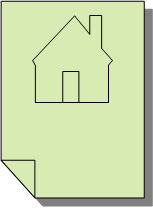
\includegraphics[width=0.25\textwidth]{figures/Homepage-icon.png}
  \end{center}
  \caption{Homepage icon}
  \label{fig:homepageicon}
\end{figure}

\begin{table}[!ht]
  \begin{center}
    \caption{Configurations tested}
    \label{tab:configstested}
    \resizebox{\columnwidth}{!}{%
    \begin{tabular}{l|c} % <-- Alignments: 1st column left, 2nd middle and 3rd right, with vertical lines in between
      \textbf{Configuration} & \textbf{Description} \\
      \hline
      1 & Simple test with one server\\
      2 & Simple test with one server\\
    \end{tabular}
    }
  \end{center}
\end{table}
\sweExpl{Testade konfigurationer}

\section{Implementation …/Modeling/Simulation/…}
\label{sec:implementationDetails}
\sweExpl{Implementering … / modellering / simulering / …}

Two commonly used simulators are:
\begin{description}[labelwidth =\widthof{\textbf{ns-2 or ns-3 simulator}}, leftmargin = !]
    \item[\textbf{Mininet}] This simulator uses traffic control (\texttt{tc}) to simulate network devices connected by links with specific bandwidth, packet loss rates, qdisc methods, etc.
    
    
    \item[\textbf{ns-2 or ns-3 simulator}] These simulators are very useful for simulating wireless communication links between moving devices. You can specify the mobility patterns of the nodes.
\end{description}

\subsection{Some examples of coding}
\engExpl{This section is simply to show some example of how you can include code in your thesis - this is not a section you would have in your thesis.}
\sweExpl{Det här avsnittet är helt enkelt för att visa ett exempel på hur du kan inkludera kod i ditt examensarbete - det här är inte ett avsnitt du skulle ha i ditt examensarbete.}

Listing~\ref{lst:helloWorldInC} shows an example of a simple program written
in C code.

\begin{lstlisting}[language={C}, caption={Hello world in C code}, label=lst:helloWorldInC]
int main() {
printf("hello, world");
return 0;
}
\end{lstlisting}


In contrast, Listing~\ref{lst:programmes} is an example of code in Python to
get a list of all of the programs at KTH.

\lstset{extendedchars=true}  %% This allows characters codes in the range 128-255
\begin{lstlisting}[language={Python}, caption={Using a python program to
    access the KTH API to get all of the programs at KTH}, label=lst:programmes]
KOPPSbaseUrl = 'https://www.kth.se'

def v1_get_programmes():
    global Verbose_Flag
    #
    # Use the KOPPS API to get the data
    # note that this returns XML
    url = "{0}/api/kopps/v1/programme".format(KOPPSbaseUrl)
    if Verbose_Flag:
        print("url: " + url)
    #
    r = requests.get(url)
    if Verbose_Flag:
        print("result of getting v1 programme: {}".format(r.text))
    #
    if r.status_code == requests.codes.ok:
        return r.text           # simply return the XML
    #
    return None
\end{lstlisting}
\FloatBarrier

\subsection{Some examples of figures in tikz}
\engExpl{This section is simply to show some example of how you can draw your own figures for in your thesis - this is not a section you would have in your thesis.}
\sweExpl{Det här avsnittet är helt enkelt för att visa ett exempel på hur du kan rita dina egna figurer i ditt examensarbete – det här är inte ett avsnitt du skulle ha i ditt examensarbete.}

These figures are just some examples to show that you can draw your own figures for in your thesis. This has two advantages: \first you do not have to worry about copyrights -- as these are your own figures and \Second the text is now readable and not simply a picture of text -- so screen readers can read the figure's contents to someone who is listening to the contents of your thesis.

\subsubsection{Azure's Form Recognizer}
\Cref{fig:processAnInvoice} shows the processing of key-value extraction from a PDF document using Azure's Form Recognizer. 

\tikzset{
    processBox/.style={rectangle, rounded corners, minimum width=3cm, minimum height=1cm,text centered, font=\sffamily, draw=black, fill=red!20},
    largeBox/.style={rectangle, rounded corners, minimum width=3cm, minimum height=4cm,text centered, draw=black}
}
\begin{figure}[!ht]
\resizebox{1.1\textwidth}{!}{%
\begin{tikzpicture}
[align=left,node distance=2cm]

\node (document) [tape,tape bend top=none,draw,font=\sffamily] {PDF\\Document};
\node (GDM) [processBox,  right=0.5cm of document] {OCR};
\node (OCRoutput) [largeBox, right=1cm of GDM] {OCR output};

\node (kvp) [tape,tape bend top=none,draw,font=\sffamily, below=0.25cm of OCRoutput.north] {key-value\\pairs};
\node (entities) [tape,tape bend top=none,draw,font=\sffamily, above=0.35cm of OCRoutput.south] {Entities};
\node (Manual) [processBox, right=1cm of kvp] {Analyze the extracted\\key-value pairs};
\draw [-latex](document) --  (GDM);
\draw [-latex](kvp) --  (Manual);
\path[ draw
     , -latex'] let \p1=(GDM.east), \p2=(kvp.west) in (GDM.east) -- +(0.25*\x2-0.25*\x1, \y1) -- +(0.5*\x2-0.5*\x1, \y2) -- (kvp.west);
\path[ draw
     , -latex'] let \p1=(GDM.east), \p2=(kvp.west), \p3=(entities.west) in (GDM.east) --  +(0.25*\x2-0.25*\x1, \y1) -- +(0.5*\x3-0.5*\x1, \y3) -- (entities.west);
\end{tikzpicture}
}
\caption{The processing of key-value extraction from a PDF document using Azure's Form Recognizer}
  \label{fig:processAnInvoice}
\end{figure}
\FloatBarrier
\subsubsection{Hyper-V with Containers}
 \Cref{fig:hyperVcontainers} shows how Hyper-V deals with containers.
 
 \tikzset{
    container/.style={rectangle, rounded corners, minimum width=2cm, minimum height=1cm,text centered, draw=black, fill=blue!20},
    containerization/.style={rectangle, rounded corners, minimum width=13.25cm, minimum height=1cm,text centered, draw=black, fill=blue!20},
    hypervisor/.style={rectangle, rounded corners, minimum width=13.25cm, minimum height=1cm,text centered, draw=black, fill=red!20},
    os/.style={rectangle, rounded corners, minimum width=13.25cm, minimum height=1cm,text centered, draw=black, fill=orange!20},
    guestos/.style={rectangle, rounded corners, minimum width=2cm, minimum height=1cm,text centered, draw=black, fill=orange!40},
    infrastructure/.style={rectangle, rounded corners, minimum width=13.25cm, minimum height=1cm,text centered, draw=black, fill=green!20},
    hos/.style={rectangle, rounded corners, minimum width=6cm, minimum height=1cm,text centered, draw=black, fill=orange!20},
    kernel/.style={rectangle, rounded corners, minimum width=6cm, minimum height=1cm,text centered, draw=black, fill=purple!20},
    services/.style={rectangle, rounded corners, minimum width=3cm, minimum height=1cm,text centered, draw=black, fill=pink!20]}
}

\begin{figure}[ht!]
    \centering
\resizebox{1\textwidth}{!}{%
\begin{tikzpicture}
[align=center,node distance=2cm]

\node (Infrastructure) [infrastructure, text width=13cm, text centered] {Infrastructure};
\node (OS1) [hos, anchor=north west, align=left, above=1.5cm of Infrastructure.north west, anchor=north west, text width=6cm, text centered] {Host OS};

\node (OS2) [hos, anchor= west, align=left, right=0.5cm of OS1.east, text width=6cm, anchor= west, text centered] {Host OS};

\node (Kernel1) [kernel, anchor=north west, align=left, above=1.5cm of OS1.north east, anchor=north east, text width=3cm, text centered] {Kernel};

\node (Kernel2) [kernel, anchor=north west, align=left, above=1.5cm of OS2.north east, anchor=north east, text width=3cm, text centered] {Kernel};

\node (ServiceA) [container, anchor=east, above=1 cm of Kernel1.east, anchor=east] {Services};
\node (AppA) [container,  left=0.25cm of ServiceA] {App 1};

\node (ServiceB) [container, anchor=east, above=1 cm of Kernel2.east, anchor=east] {Services};
\node (AppB) [container,  left=0.25cm of ServiceB] {App 2};
%\node (AppC) [container,  right=0.25cm of AppB] {App 3};

\draw[black,thick,dashed] ($(OS2.north west)+(-0.3,3.75)$)  rectangle ($(OS2.south east)+(0.5,-0.3)$);
\node[text width=5cm, text=red, above=0.1cm of ServiceB] 
    {\textbf{Container}};

\draw[red,thick,dotted] ($(Kernel2.north west)+(-0.3,1.6)$)  rectangle ($(Kernel2.south east)+(0.3,-0.3)$);
\node[text width=5cm, text=black, above=0.8cm of ServiceB] 
    {\textbf{VM}};
\end{tikzpicture}
}
    \caption{Hyper-V with containers}
    \label{fig:hyperVcontainers}
\end{figure}
\FloatBarrier
\subsubsection{\glsfmtshort{VM} versus Containers}
\Cref{fg:vmsVersusContainers} shows a comparison of virtual machines (VMs) versus containers.

\begin{figure*}[ht!]
    \centering
    \begin{subfigure}[t]{0.5\textwidth}
        \centering
\resizebox{1\textwidth}{!}{%
\begin{tikzpicture}
[align=left,node distance=2cm]

\node (AppA) [container,align=left] {App 1};
\node (AppB) [container,  right=0.25cm of AppA] {App 2};
\node (AppC) [container,  right=0.25cm of AppB] {App 3};

\node (GosA) [guestos,align=left,  below=0.25cm of AppA.south west,anchor=north west] {Guest OS};
\node (GosB) [guestos,  right=0.25cm of GosA] {Guest OS};
\node (GosC) [guestos,  right=0.25cm of GosB] {Guest OS};

\draw [decoration={brace,amplitude=0.5em},decorate, ultra thick,gray, transform canvas={xshift = 0.5cm}]
       (AppC.north -| AppC.east) -- (GosC.south -| AppC.east);
\node[text width=5cm,  right=1cm of GosC.north east] 
    {\textbf{VMs}};

\node (Hypervisor) [hypervisor, anchor=north west, align=left, below=0.25cm of GosA.south west, anchor=north west, text width=13cm, text centered] {Hypervisor};

\node (OS) [os, anchor=north west, align=left, below=0.25cm of Hypervisor.south west, anchor=north west, text width=13cm, text centered] {Host OS};

\node (Infrastructure) [infrastructure, anchor=north west, align=left, below=0.25cm of OS.south west, anchor=north west, text width=13cm, text centered] {Infrastructure};


\end{tikzpicture}
}
        \caption{VM}
    \end{subfigure}%
    ~ 
    \begin{subfigure}[t]{0.5\textwidth}
        \centering
        \resizebox{1\textwidth}{!}{%
\begin{tikzpicture}
[align=left,node distance=2cm]

\node (AppA) [container,align=left] {App 1};
\node (AppB) [container,  right=0.25cm of AppA] {App 2};
\node (AppC) [container,  right=0.25cm of AppB] {App 3};
\node[text width=5cm,  right=0.25cm of AppC] 
    {\textbf{Apps running in Containers}};


\node (Containerization) [containerization, anchor=north west, align=left, below=0.25cm of AppA.south west, anchor=north west, text width=13cm, text centered] {Docker Engine};

\node (OS) [os, anchor=north west, align=left, below=0.25cm of Containerization.south west, anchor=north west, text width=13cm, text centered] {Host OS};

\node (Infrastructure) [infrastructure, anchor=north west, align=left, below=0.25cm of OS.south west, anchor=north west, text width=13cm, text centered] {Infrastructure};


\end{tikzpicture}
}
        \caption{Containers}
    \end{subfigure}
    \caption{Virtual machines (VMs) versus Containers}
    \label{fg:vmsVersusContainers}
\end{figure*}


\cleardoublepage

\chapter{Results and Analysis}
    \label{ch:results_and_analysis}
    \sweExpl{svensk: Resultat och Analys}

\engExpl{Sometimes this is split into two chapters.\\Keep in mind: How you are going to evaluate what you have done? What are your metrics?\\Analysis of your data and proposed solution\\Does this meet the goals which you had when you started?}

In this chapter, we present the results and discuss them.

\sweExpl{I detta kapitel presenterar vi resultaten och diskutera dem.\\Ibland delas detta upp i två kapitel.\\Hur du ska utvärdera vad du har gjort? Vad är din statistik?\\Analys av data och föreslagen lösning\\Innebär detta att uppfyllelse av de mål som du hade när du började?}

\section{Major results}
\sweExpl{Huvudsakliga resultat}

Some statistics of the delay measurements are shown in Table~\ref{tab:delayMeasurements}.
The delay has been computed from the time the GET request is received until the response is sent.

\sweExpl{Lite statistik av fördröjningsmätningarna visas i Tabell~\ref{tab:delayMeasurements}. Förseningen har beräknats från den tidpunkt då begäran GET tas emot fram till svaret skickas.}

\begin{table}[!ht]
  \begin{center}
    \caption{Delay measurement statistics}
    \label{tab:delayMeasurements}
    \begin{tabular}{l|S[table-format=4.2]|S[table-format=3.2]} % <-- Alignments: 1st column left, 2nd middle and 3rd right, with vertical lines in between
      \textbf{Configuration} & \textbf{Average delay (ns)} & \textbf{Median delay (ns)}\\
      \hline
      1 & 467.35 & 450.10\\
      2 & 1687.5 & 901.23\\
    \end{tabular}
  \end{center}
\end{table}

Table \ref{tab:ping_results} shows the measurement of round trip times from four hosts to and from a server.
\begin{table}[ht!]
\caption[RTT for 4 hosts]{Result for the ping measurements of RTT for 4 hosts} 
\label{tab:ping_results}
\vspace{1em}
\centering
\begin{tabular}{l *{4}{S[table-format=2.3]}}
{} & \multicolumn{4}{c}{host to server RTT in ms} \\
\cmidrule{2-5}
Host & \multicolumn{1}{c}{min}  & \multicolumn{1}{c}{avg} & \multicolumn{1}{c}{max} & \multicolumn{1}{c}{mdev} \\
\midrule
h1 & 5.625 & 5.625 & 5.625 & 0.0 \\
h2 & 2.909 & 2.909 & 1.909 & 0.0 \\
h3 & 5.007 & 5.007 & 5.007 & 0.0 \\
h4 & 2.308 & 2.308 & 2.308 & 0.0 \\
\midrule
\end{tabular}
\end{table}
\FloatBarrier

\sweExpl{Fördröj mätstatistik}
\sweExpl{Konfiguration | Genomsnittlig fördröjning (ns) | Median fördröjning (ns)}

Figure \ref{fig:processing_vs_payload_length} shows an example of the performance as measured in the experiments.

\begin{figure}[!ht]
% GNUPLOT: LaTeX picture
\setlength{\unitlength}{0.240900pt}
\ifx\plotpoint\undefined\newsavebox{\plotpoint}\fi
\begin{picture}(1500,900)(0,0)
\sbox{\plotpoint}{\rule[-0.200pt]{0.400pt}{0.400pt}}%
\put(171.0,131.0){\rule[-0.200pt]{4.818pt}{0.400pt}}
\put(151,131){\makebox(0,0)[r]{ 1.5}}
\put(1419.0,131.0){\rule[-0.200pt]{4.818pt}{0.400pt}}
\put(171.0,212.0){\rule[-0.200pt]{4.818pt}{0.400pt}}
\put(151,212){\makebox(0,0)[r]{ 2}}
\put(1419.0,212.0){\rule[-0.200pt]{4.818pt}{0.400pt}}
\put(171.0,292.0){\rule[-0.200pt]{4.818pt}{0.400pt}}
\put(151,292){\makebox(0,0)[r]{ 2.5}}
\put(1419.0,292.0){\rule[-0.200pt]{4.818pt}{0.400pt}}
\put(171.0,373.0){\rule[-0.200pt]{4.818pt}{0.400pt}}
\put(151,373){\makebox(0,0)[r]{ 3}}
\put(1419.0,373.0){\rule[-0.200pt]{4.818pt}{0.400pt}}
\put(171.0,454.0){\rule[-0.200pt]{4.818pt}{0.400pt}}
\put(151,454){\makebox(0,0)[r]{ 3.5}}
\put(1419.0,454.0){\rule[-0.200pt]{4.818pt}{0.400pt}}
\put(171.0,534.0){\rule[-0.200pt]{4.818pt}{0.400pt}}
\put(151,534){\makebox(0,0)[r]{ 4}}
\put(1419.0,534.0){\rule[-0.200pt]{4.818pt}{0.400pt}}
\put(171.0,615.0){\rule[-0.200pt]{4.818pt}{0.400pt}}
\put(151,615){\makebox(0,0)[r]{ 4.5}}
\put(1419.0,615.0){\rule[-0.200pt]{4.818pt}{0.400pt}}
\put(171.0,695.0){\rule[-0.200pt]{4.818pt}{0.400pt}}
\put(151,695){\makebox(0,0)[r]{ 5}}
\put(1419.0,695.0){\rule[-0.200pt]{4.818pt}{0.400pt}}
\put(171.0,776.0){\rule[-0.200pt]{4.818pt}{0.400pt}}
\put(151,776){\makebox(0,0)[r]{ 5.5}}
\put(1419.0,776.0){\rule[-0.200pt]{4.818pt}{0.400pt}}
\put(171.0,131.0){\rule[-0.200pt]{0.400pt}{4.818pt}}
\put(171,90){\makebox(0,0){ 0}}
\put(171.0,756.0){\rule[-0.200pt]{0.400pt}{4.818pt}}
\put(298.0,131.0){\rule[-0.200pt]{0.400pt}{4.818pt}}
\put(298,90){\makebox(0,0){ 10}}
\put(298.0,756.0){\rule[-0.200pt]{0.400pt}{4.818pt}}
\put(425.0,131.0){\rule[-0.200pt]{0.400pt}{4.818pt}}
\put(425,90){\makebox(0,0){ 20}}
\put(425.0,756.0){\rule[-0.200pt]{0.400pt}{4.818pt}}
\put(551.0,131.0){\rule[-0.200pt]{0.400pt}{4.818pt}}
\put(551,90){\makebox(0,0){ 30}}
\put(551.0,756.0){\rule[-0.200pt]{0.400pt}{4.818pt}}
\put(678.0,131.0){\rule[-0.200pt]{0.400pt}{4.818pt}}
\put(678,90){\makebox(0,0){ 40}}
\put(678.0,756.0){\rule[-0.200pt]{0.400pt}{4.818pt}}
\put(805.0,131.0){\rule[-0.200pt]{0.400pt}{4.818pt}}
\put(805,90){\makebox(0,0){ 50}}
\put(805.0,756.0){\rule[-0.200pt]{0.400pt}{4.818pt}}
\put(932.0,131.0){\rule[-0.200pt]{0.400pt}{4.818pt}}
\put(932,90){\makebox(0,0){ 60}}
\put(932.0,756.0){\rule[-0.200pt]{0.400pt}{4.818pt}}
\put(1059.0,131.0){\rule[-0.200pt]{0.400pt}{4.818pt}}
\put(1059,90){\makebox(0,0){ 70}}
\put(1059.0,756.0){\rule[-0.200pt]{0.400pt}{4.818pt}}
\put(1185.0,131.0){\rule[-0.200pt]{0.400pt}{4.818pt}}
\put(1185,90){\makebox(0,0){ 80}}
\put(1185.0,756.0){\rule[-0.200pt]{0.400pt}{4.818pt}}
\put(1312.0,131.0){\rule[-0.200pt]{0.400pt}{4.818pt}}
\put(1312,90){\makebox(0,0){ 90}}
\put(1312.0,756.0){\rule[-0.200pt]{0.400pt}{4.818pt}}
\put(1439.0,131.0){\rule[-0.200pt]{0.400pt}{4.818pt}}
\put(1439,90){\makebox(0,0){ 100}}
\put(1439.0,756.0){\rule[-0.200pt]{0.400pt}{4.818pt}}
\put(171.0,131.0){\rule[-0.200pt]{0.400pt}{155.380pt}}
\put(171.0,131.0){\rule[-0.200pt]{305.461pt}{0.400pt}}
\put(1439.0,131.0){\rule[-0.200pt]{0.400pt}{155.380pt}}
\put(171.0,776.0){\rule[-0.200pt]{305.461pt}{0.400pt}}
\put(30,453){\rotatebox{-270}{\makebox(0,0){Processing time (ms)}}}
\put(805,29){\makebox(0,0){Payload size (bytes)}}
\put(868.0,131.0){\rule[-0.200pt]{0.400pt}{84.074pt}}
\put(995.0,131.0){\rule[-0.200pt]{0.400pt}{98.287pt}}
\put(1173.0,131.0){\rule[-0.200pt]{0.400pt}{118.041pt}}
\put(1325.0,131.0){\rule[-0.200pt]{0.400pt}{134.904pt}}
\put(1350.0,131.0){\rule[-0.200pt]{0.400pt}{137.795pt}}
\put(1439.0,131.0){\rule[-0.200pt]{0.400pt}{155.380pt}}
\end{picture}
\caption[A GNUplot figure]{Processing time vs. payload length}\vspace{0.5cm}
\label{fig:processing_vs_payload_length}
\end{figure}
\FloatBarrier		

Given these measurements, we can calculate our processing bit rate as the inverse of the time it takes to process an additional byte divided by 8 bits per byte:

\[
	\text{bit rate} = \frac{1}{\frac{\text{time}_{\text{byte}}}{8}} = 20.03 \quad kb/s
\] 

\Cref{tab:majorMarkupLMDetailedResult} shows another table in which some values have been set in bold (using \textbackslash B) to emphasize them. Note how the \texttt{S} formatting has been modified so that it considers the weight of the characters and this is able to decimal align even these hold-faced numbers with the numbers in the column above them.

\begin{table}[!ht]
    \centering
    \caption{Median values of sandwich attributes}
    \label{tab:majorMarkupLMDetailedResult}
    \begin{tabular}{l *{2}{S[detect-weight,mode=text,table-format=3.2]}}
        & \multicolumn{2}{c}{\textbf{sites}}\\
        \cmidrule{2-3}
        \textbf{Attribute} & \textbf{A} & \textbf{B} \\
        \midrule
        price (in SEK) & 36.5 & 71.3 \\
        protean (g) & 97.2 & 100.0 \\
        salt (mg) & 9.7 & 9.3 \\
        \hline
        \textbf{Average customer rating in \%} & \B 82.2 & \B 89.9 \\
        \midrule
    \end{tabular}
\end{table}
\FloatBarrier


\Needspace*{4\baselineskip}
\Cref{fig:stackedrust} shows a stacked bar chart using pgfplots. It illustrates how easy it is to take a set of data and make a stacked bar plot. One of the features is the shifted values -- this is very useful when the bar itself is too small to put the value into.

\pgfplotstableread{
Label Numbers  Refs  Struct/Enum  Heap  Arrays
cratesio 70.04 19.83 8.31 1.3 0.52
librs 49.26 30.49 10.80 7.92 1.53
rustc 55.01 24.80 11.54 6.16 2.49
}\testdata


\pgfkeys{
    /pgf/number format/.cd,
    fixed,
    fixed zerofill,
    precision=2
}
\begin{figure}[ht!]
    \centering
    \scalebox{0.9}{
    \begin{tikzpicture}
    \begin{axis}[
        ybar stacked,
        %reverse legend,
        reverse legend=false,
        %https://tex.stackexchange.com/questions/88892/pgfplots-bar-plot-spacing-inbetween-bars
        enlarge x limits=0.4,
	    bar width=45pt,
        /pgfplots/nodes near coords*/.append style={
        every node near coord/.style={
            color=black,
            font=\small,
            name=X,
%            shift={    
%                (50pt,25pt)
%                },
            xshift={50pt},
                yshift ={
                ifthenelse((\plotnum == 4), 30pt,20pt)},
            },
            scatter/@post marker code/.append code={
                \node(Y){};
                \draw(X)--(Y.center);
            }
        },
	    nodes near coords,
        bar shift=5pt,
        ymin=0,
        ymax=115,
        xtick=data,
        width=1\textwidth,
        legend style={draw=none},
        legend image post style={scale=2.0},
        legend style={
            at={(0.5,-0.2)},
            anchor=north,
            legend columns=-2,
            font=\large,
            %mark size=20pt,
        },
        ylabel=Percentage points (\%),
        xticklabels from table={\testdata}{Label},
        xticklabel style={rotate=30},
    ]
    \addplot  table [y=Numbers, meta=Label, x expr=\coordindex] {\testdata};
    \addlegendentry{Numbers}
    \addplot table [y=Refs, meta=Label, x expr=\coordindex] {\testdata};
    \addlegendentry{Refs}
    \addplot  table [y=Struct/Enum, meta=Label, x expr=\coordindex] {\testdata};
    \addlegendentry{Struct/Enum}
    \addplot  table [y=Heap, meta=Label, x expr=\coordindex] {\testdata};
    \addlegendentry{Heap}
    \addplot  table [y=Arrays, meta=Label, x expr=\coordindex] {\testdata};
    \addlegendentry{Arrays}
    \end{axis}
    \end{tikzpicture}}
\caption{Rust types distribution for the compiler, crates.io, and lib.rs.
(percentage) - appears here with the permission of the author - see the thesis at \url{https://urn.kb.se/resolve?urn=urn\%3Anbn\%3Ase\%3Akth\%3Adiva-332124}}
\label{fig:stackedrust}
\end{figure}
\FloatBarrier



\section{Reliability Analysis}
\sweExpl{Analys av tillförlitlighet\\
Tillförlitlighet i metod och data}

\section{Validity Analysis}
\sweExpl{Analys av validitet\\
Validitet i metod och data}

\cleardoublepage
\chapter{Discussion}
\label{ch:discussion}
\sweExpl{Diskussion\\
Förbättringsförslag?}
\generalExpl{This can be a separate chapter or a section in the previous chapter.}

\cleardoublepage

\chapter{Conclusions and Future work}
    \label{ch:conclusions_and_future_work}
    \sweExpl{Slutsats och framtida arbete}

\generalExpl{Add text to introduce the subsections of this chapter.}

\section{Conclusions}
\label{sec:conclusions}
\sweExpl{Slutsatser}
\engExpl{Describe the conclusions (reflect on the whole introduction given in Chapter 1).}


  
\engExpl{Discuss the positive effects and the drawbacks.\\
Describe the evaluation of the results of the degree project.\\
Did you meet your goals?\\
What insights have you gained?\\
What suggestions can you give to others working in this area?\\
If you had it to do again, what would you have done differently?}

\sweExpl{Uppfyllde du dina mål?\\
Vilka insikter har du fått?\\
Vilka förslag kan du ge till andra som arbetar inom detta område?
Om du skulle göra detta igen, vad skulle du ha gjort annorlunda?}

\section{Limitations}
\label{sec:limitations}
\sweExpl{Begränsande faktorer\\Vad gjorde du som begränsade dina ansträngningar? Vilka är begränsningarna i dina resultat?}
\engExpl{What did you find that limited your efforts? What are the limitations of your results?}


\section{Future work}
\label{sec:futureWork}
\sweExpl{Vad du har kvar ogjort?\\Vad är nästa självklara saker som ska göras?\\Vad tips kan du ge till nästa person som kommer att följa upp på ditt arbete?}
\engExpl{Describe valid future work that you or someone else could or should do.\\
Consider: What you have left undone? What are the next obvious things to be done? What hints can you give to the next person who is going to follow up on your work?}



Due to the breadth of the problem, only some of the initial goals have been
met. In these section we will focus on some of the remaining issues that
should be addressed in future work. ...

\subsection{What has been left undone?}
\label{what-has-been-left-undone}

The prototype does not address the third requirment, \ie a yearly unavailability of less than 3 minutes; this remains an open problem. ...

\subsubsection{Cost analysis}
\generalExpl{Example of a missing component}
The current prototype works, but the performance from a cost perspective makes this an impractical solution. Future work must reduce the cost of this solution; to do so, a cost analysis needs to first be done. ...

\subsubsection{Security}
\generalExpl{Example of a missing component}
A future research effort is needed to address the security holes that results from using a self-signed certificate. Page filling text mass. Page filling text mass. ...


\subsection{Next obvious things to be done}

In particular, the author of this thesis wishes to point out xxxxxx remains as a problem to be solved. Solving this problem is the next thing that should be done. ...

\section{Reflections}
\label{sec:reflections}
\sweExpl{Reflektioner}
\sweExpl{Vilka är de relevanta ekonomiska, sociala, miljömässiga och etiska aspekter av ditt arbete?}
\engExpl{What are the relevant economic, social,
  environmental, and ethical aspects of your work?
}



One of the most important results is the reduction in the amount of
energy required to process each packet while at the same time reducing the
time required to process each packet.

The thesis contributes to the \gls{UN}\enspace\glspl{SDG} numbers 1 and 9 by
xxxx. 


%%%%%%%%%%%%%%%%%%%%%%%%%%%%%%%%%%%%%%%%%%%%%%%%%%%%%%%%%%%%%%%%%%%%%%%%%%%%%%%%%%%%%%%%
%%                                 REFERENCES
%%%%%%%%%%%%%%%%%%%%%%%%%%%%%%%%%%%%%%%%%%%%%%%%%%%%%%%%%%%%%%%%%%%%%%%%%%%%%%%%%%%%%%%%
\noindent\rule{\textwidth}{0.4mm}
\engExpl{In the references, let Zotero or other tool fill this in for you. I suggest an extended version of the IEEE style, to include URLs, DOIs, ISBNs, etc., to make it easier for your reader to find them. This will make life easier for your opponents and examiner. \\IEEE Editorial Style Manual: \url{https://www.ieee.org/content/dam/ieee-org/ieee/web/org/conferences/style_references_manual.pdf}}

\cleardoublepage

% Print the bibliography (and make it appear in the table of contents)
\renewcommand{\bibname}{References}

\ifbiblatex
    %\typeout{Biblatex current language is \currentlang}
    \printbibliography[heading=bibintoc]
\else
    \phantomsection  % make it include a hyperref - see https://tex.stackexchange.com/a/98995
    \addcontentsline{toc}{chapter}{References}
    \bibliography{references}
\fi

%%%%%%%%%%%%%%%%%%%%%%%%%%%%%%%%%%%%%%%%%%%%%%%%%%%%%%%%%%%%%%%%%%%%%%%%%%%%%%%%%%%%%%%%
%%                                 APPENDIX
%%%%%%%%%%%%%%%%%%%%%%%%%%%%%%%%%%%%%%%%%%%%%%%%%%%%%%%%%%%%%%%%%%%%%%%%%%%%%%%%%%%%%%%%
%% If you do not have an appendix, do not include the \textbackslash cleardoublepage command below; otherwise, the last page number in the metadata will be one too large.}
\cleardoublepage

\appendix
\renewcommand{\chaptermark}[1]{\markboth{Appendix \thechapter\relax:\thinspace\relax#1}{}}

\chapter{Supporting materials}
    \label{sec:supportingMaterial}
    This appendix contains the system architecture diagrams, for both the legacy system and the Apache Iceberg version.

\cleardoublepage

\chapter{Something Extra}
    This appendix contains the writing diagrams, showing the barplots and the schema with all the information the writing experiments performed on the different systems.

% Include an example of using nomenclature
\ifnomenclature
\cleardoublepage

\chapter{Main equations}
    \label{ch:NomenclatureExamples}
    This appendix contains the reading diagrams, showing the barplots and the schema with all the information the reading experiments performed on the different systems.


\cleardoublepage

%% The following label is necessary for computing the last page number of the body of the report to include in the "For DIVA" information
\label{pg:lastPageofMainmatter}

\cleardoublepage

%%%%%%%%%%%%%%%%%%%%%%%%%%%%%%%%%%%%%%%%%%%%%%%%%%%%%%%%%%%%%%%%%%%%%%%%%%%%%%%%%%%%%%%%
%%                                 FOR DIVA MATERIAL
%%%%%%%%%%%%%%%%%%%%%%%%%%%%%%%%%%%%%%%%%%%%%%%%%%%%%%%%%%%%%%%%%%%%%%%%%%%%%%%%%%%%%%%%
\clearpage\thispagestyle{empty}\mbox{} % empty page with backcover on the other side
\kthbackcover
\fancyhead{}  % Do not use header on this extra page or pages
\section*{€€€€ For DIVA €€€€}
\lstset{numbers=none} %% remove any list line numbering
\divainfo{pg:lastPageofPreface}{pg:lastPageofMainmatter}

% If there is an acronyms.tex file,
% add it to the end of the For DIVA information
% so that it can be used with the abstracts
% Note that the option "nolol" stops it from being listed in the List of Listings

% The following bit of ugliness is because of the problems PDFLaTeX has handling a non-breaking hyphen
% unless it is converted to UTF-8 encoding.
% If you do not use such characters in your acronyms, this could be simplified.
\ifxeorlua
\IfFileExists{lib/acronyms.tex}{
\section*{acronyms.tex}
\lstinputlisting[language={[LaTeX]TeX}, nolol, basicstyle=\ttfamily\color{black},
commentstyle=\color{black}, backgroundcolor=\color{white}]{lib/acronyms.tex}
}
{}
\else
\IfFileExists{lib/acronyms-for-pdflatex.tex}{
\section*{acronyms.tex}
\lstinputlisting[language={[LaTeX]TeX}, nolol, basicstyle=\ttfamily\color{black},
commentstyle=\color{black}, backgroundcolor=\color{white}]{lib/acronyms-for-pdflatex.tex}
}
{}
\fi

\end{document}
